\documentclass[sigconf,review,anonymous]{acmart}

%% ACM metadata — The Web Conference 2027 (WWW '27), Dublin.
%% Abstracts 2026-10-18, full papers 2026-10-25 (AoE). Page limit not yet published
%% at the time of writing; verify against the official CFP before submitting.
%% WWW review is double-blind: `anonymous` strips authors and affiliations.
%% Suppress copyright/ISBN/DOI and the ACM Reference Format during review;
%% replace with the eRights values at camera-ready.
\setcopyright{none}
\settopmatter{printacmref=false}
\copyrightyear{2027}
\acmYear{2027}
\acmConference[WWW '27]{Proceedings of the ACM Web Conference 2027}{April 2027}{Dublin, Ireland}

%% Additional packages (not bundled in acmart)
\usepackage{tikz-cd}
\usepackage{tikz}
\usetikzlibrary{positioning,arrows.meta,shapes.geometric,fit,backgrounds}
\usepackage{pgfplots}
\pgfplotsset{compat=1.18}
\usepgfplotslibrary{fillbetween}
\usepackage{multicol}
\usepackage{booktabs}

%% Permissive float fractions: allow 2 wide tables to share a page
\renewcommand{\dbltopfraction}{0.95}
\renewcommand{\dblfloatpagefraction}{0.7}
\renewcommand{\topfraction}{0.9}
\renewcommand{\floatpagefraction}{0.7}
\setcounter{topnumber}{3}
\setcounter{dbltopnumber}{3}
\setcounter{totalnumber}{4}

%% TikZ styles for figure skeletons (replace with PPT-rendered PNGs in camera-ready)
\tikzset{
  fbox/.style={draw, rounded corners=2pt, minimum height=6mm, align=center, font=\footnotesize, inner sep=2pt},
  fnode/.style={fbox, fill=blue!5},
  fnoter/.style={fbox, fill=orange!10},
  fop/.style={fbox, fill=green!8},
  farr/.style={-{Latex[length=1.5mm]}, thick},
  fdash/.style={-{Latex[length=1.5mm]}, thick, dashed},
}

%%% Title
\title{What Consolidation Destroys: Measuring Information Loss in LLM-Maintained Hierarchical User Memory}

%%% Authors — hidden by the `anonymous` class option for WWW double-blind review.
\author{Junguel Lee}
\affiliation{%
  \institution{Naver Corp}
  \city{Seongnam-si}
  \country{South Korea}
}
\email{junguel.lee@navercorp.com}

\author{Jungseok Lee}
\affiliation{%
  \institution{Naver Corp}
  \city{Seongnam-si}
  \country{South Korea}
}
\email{jungseok.lee@navercorp.com}

\author{Sangam Lee}
\affiliation{%
  \institution{Yonsei University}
  \city{Seoul}
  \country{South Korea}
}
\email{salee@yonsei.ac.kr}

\author{Jihoon Choi}
\authornote{Corresponding author.}
\affiliation{%
  \institution{Naver Corp}
  \city{Seongnam-si}
  \country{South Korea}
}
\email{jh.choi@navercorp.com}

\author{Changhoe Kim}
\authornotemark[1]
\affiliation{%
  \institution{Naver Corp}
  \city{Seongnam-si}
  \country{South Korea}
}
\email{andres.chkim@navercorp.com}

\begin{abstract}
Hierarchical memory systems for LLM agents periodically consolidate their own contents: sibling notes are merged, shared traits are promoted to a parent, stale nodes are pruned. Consolidation is normally justified by footprint and evaluated by downstream accuracy, so what it removes is never observed directly. We deploy such a memory as the persistent user model of a large Korean web map service and measure the removal itself.

We track every keyword in a child note across one consolidation pass and classify it as \emph{retained}, \emph{lifted} to the parent, or \emph{lost} entirely. On 500 production memory trees, unguarded trait elevation with gemma-4-31b loses \(25.3\%\) of child keywords --- counting only those absent from the surrounding prose as well --- and loses them even where siblings share no keyword at all and nothing needs to move. That stratum still loses \(18.0\%\): the deletion looks collateral to the rewrite rather than a consequence of compression.

Three findings follow. First, the magnitude is a property of the backbone, not of the method: across three models the same prompt ranges from \(34\%\) keyword compression to \(5\%\) \emph{inflation}, and the prompt-level guard that is decisive on one model slightly but significantly \emph{increases} loss on the model we actually deployed. Second, that guard protects the wrong tokens --- place and brand names survive above their base rate, while what is lost in bulk is category vocabulary and, at \(2.4\times\) its base rate, the behavioural evidence grounding each claim; a guard rewritten from the measured loss profile cuts loss from \(0.181\) to \(0.160\) (\(p<0.0001\)). Third, sibling merging, which prior work leaves unexamined, turns out to relocate rather than delete: it appears to contribute roughly a quarter of total loss under a same-path instrument and \(+0.007\) under one that follows relocation.

The loss is not recovered downstream: over \(70\%\) of lost keywords are also absent from the regenerated persona, and not because a different subtree was selected. On a leak-free held-out MCQ, accuracy on the development half orders inversely to loss (\(0.452\) to \(0.484\)) but no pairwise difference is significant at \(N{=}500\), so we report consolidation as a compression mechanism whose information cost is now measurable and, on one backbone, reducible, not as an accuracy lever. Every loss result was developed on one half of each snapshot and confirmed on a reserved half opened once (the instrument was corrected afterwards and both halves recomputed): the aggregate loss measurements replicate to within \(0.003\), and the accuracy null replicates too.
\end{abstract}

%% CCS concepts (required by acmart for papers > 2 pages)
\begin{CCSXML}
<ccs2012>
   <concept>
       <concept_id>10002951.10003317.10003347.10003350</concept_id>
       <concept_desc>Information systems~Recommender systems</concept_desc>
       <concept_significance>500</concept_significance>
   </concept>
   <concept>
       <concept_id>10010147.10010178.10010179</concept_id>
       <concept_desc>Computing methodologies~Natural language processing</concept_desc>
       <concept_significance>300</concept_significance>
   </concept>
   <concept>
       <concept_id>10010147.10010178.10010187</concept_id>
       <concept_desc>Computing methodologies~Knowledge representation and reasoning</concept_desc>
       <concept_significance>300</concept_significance>
   </concept>
</ccs2012>
\end{CCSXML}
\ccsdesc[500]{Information systems~Recommender systems}
\ccsdesc[300]{Computing methodologies~Natural language processing}
\ccsdesc[300]{Computing methodologies~Knowledge representation and reasoning}

\keywords{user modeling, personalization, memory-augmented LLM agents, memory consolidation, information loss}

\begin{document}
\maketitle


%% ============================================================
%% INTRODUCTION
%% ============================================================
\section{Introduction}

Web services increasingly hand the user model behind their personalization to LLM agents that read it and keep it current; this paper measures what that upkeep destroys, in a deployed map and place-search service (\(2.0\text{M}\) distinct users over five weeks). In POI (Point-of-Interest)-centric services the model must capture which place types a user prefers and how they visit. Real POI logs make that hard: they are large-scale and noisy, explicit signals such as reviews are sparse, and implicit ones are pervasive but ambiguous~\cite{proex}. Neither of the standard constructions fits. Full-context prompting hits context limits and lost-in-the-middle effects~\cite{lost-in-the-middle}: strong on factual recall (\(92.85\%\) on LoCoMo~\cite{beyond-context-window}) but behind a compact agentic memory on implicit personalization (\(45.6\%\) for GPT-5-Chat vs.\ \(55.2\%\)~\cite{personamem-v2}), at much higher cost. Retrieval over flat chunks~\cite{dpr,contriever} avoids the limit but cannot move between fine-grained categories and higher-level tendencies such as a dining-focused lifestyle. Our own measurements narrow this motivation: at the size our deployed memory reaches, flattening it away costs nothing downstream and selecting from it costs a great deal (Section~\ref{sec:delivery}); the hierarchy buys bounded read cost and a place for a maintenance policy, not accuracy.

We deploy a POI-centric Hierarchical Note-based Memory and a Memory Agent that maintains it (Figure~\ref{fig:overview} in Appendix~\ref{app:motivation} gives a worked example). The memory aggregates POI activities into topic-specific notes via LLM reasoning and organizes them in a three-level POI taxonomy.

Every such system must eventually consolidate, or its trees grow without bound: on our deployment, where consolidation has effectively not run, notes per user rise \(16.4\%\) and keywords \(29.5\%\) per update cycle. What consolidation costs to stop that has not been measured. Prior systems justify it by footprint and validate it by downstream accuracy~\cite{mem0,personamem-v2}, which leaves the operation unobserved: a consolidation that quietly discards half the evidence and one that losslessly reorganizes it are indistinguishable if both shrink the tree and neither moves an accuracy number carrying its own noise. 

We instrument the operation rather than its consequences, following each keyword through one consolidation pass on deployed memory. The resulting picture is not the one the design assumed, and not the same on every backbone.

Our contributions are:
\begin{itemize}
    \item \textbf{A direct measure of consolidation loss.} Every child keyword is classified as retained, lifted, or lost across one pass: the operation is observed, not inferred from downstream scores, and needs no labels.
    \item \textbf{Evidence that consolidation deletes rather than compresses.} Users whose siblings share no keyword --- where promotion has nothing to promote --- still lose nearly a fifth of their child keywords, and loss rises monotonically with the amount genuinely shared.
    \item \textbf{Backbone dependence, with a sign change.} The same prompt on the same trees ranges from heavy compression to net inflation across three models, and the guard decisive on one significantly increases loss on another --- the one we deployed. 
    \item \textbf{A guard derived from measurement, and a mis-attributed source of loss.} The deployed guard names tokens that were never at risk; rewriting it around the measured loss profile reduces loss further at no additional inference cost. Merging, which prior work ignores, turns out to relocate rather than delete; a same-path instrument reports it as roughly a quarter of all loss.
    \item \textbf{Propagation to the consumed artifact, and a larger loss beside it.} Over \(70\%\) of the keywords consolidation removes also vanish from the regenerated persona and not because a different subtree was selected. Measuring the delivery path itself against the raw notes then found it the more expensive operation, by roughly a factor of six: selection and synthesis together cost \(+0.190\) accuracy, three quarters of the gain the deployed memory delivers over an empty persona.
    \item \textbf{Confirmation on reserved data.} Each snapshot was split in half; every loss comparison was developed on one half and verified on the other (with one post-hoc correction, Section~\ref{sec:data}), including the guard derived from the development half.
\end{itemize}


%% ============================================================
%% RELATED WORK
%% ============================================================
\section{Related Work}
\label{sec:related}

\paragraph{Memory architectures and their maintenance operations.}
Building on LLM-agent frameworks~\cite{react,reflexion,generative-agents}, agent memory varies in structure (flat vs.\ hierarchical) and in maintenance (append-only vs.\ actively managed; cf.~\cite{memory-survey}). One family rewrites or discards what it holds. Mem0~\cite{mem0} issues per-item update and delete decisions over a flat list; MemGPT~\cite{memgpt} pages content out of context; MemoryBank~\cite{memorybank} applies Ebbinghaus-curve forgetting; PersonaMem-v2~\cite{personamem-v2} trains a 4B agent to rewrite a single compact persona memory as conversations arrive, and beats GPT-5-Chat (\(55.2\%\) vs.\ \(45.6\%\)) at \(16\times\) fewer tokens than the full history. The other family does not contract: A-Mem~\cite{amem} creates, links and updates notes with no described merge or prune step, EMem~\cite{emem} stores information in a non-compressive event graph and exceeds full-context quality on LoCoMo with ${\sim}32\times$ fewer tokens, and HippoRAG~\cite{hipporag} indexes through a knowledge graph. PersonaMem~\cite{personamem} benchmarks dynamic user profiling. Our deployment belongs to the first family, with dynamic routing, trait elevation and a third extraction axis --- and this paper is about what its rewriting step removes.

\paragraph{The measurement gap.}
Contraction is justified by footprint and validated by downstream task scores, a pairing that cannot distinguish a step that reorganizes losslessly from one that discards evidence: both shrink the store, and a noisy task score will not separate them. We know of no benchmark in this line that reports what a maintenance pass removed, only what the memory scored afterwards, so we instrument the operation itself.

\paragraph{Faithfulness under abstraction.}
Trait elevation is abstractive summarization applied to a system's own state, and abstractive summarizers are known to hallucinate and distort source content~\cite{maynez-faithfulness,hallucination-survey}. The memory setting is harsher: a summarizer leaves its source intact, so a failure is recoverable by re-reading, whereas a memory agent overwrites, so what one pass discards is absent from every later read, and there is no source to check against at maintenance time --- which is why the loss goes unnoticed. Input-side prompt compression~\cite{llmlingua} maps the same frontier for transient context; ours is persistent state, where each pass compresses an already-compressed artifact.

\paragraph{Prompt sensitivity and backbone dependence.}
LLM behaviour shifts under prompt changes a human would call cosmetic~\cite{formatspread}, motivating evaluation across multiple prompts~\cite{multiprompt}. That literature measures how a prompt's \emph{score} moves; we report the same fragility in what a prompt \emph{destroys}, across backbones rather than formats: with the prompt and the trees held fixed, one model compresses by a third while another inflates, and a guard that is decisive on the first significantly increases loss on the second.

\paragraph{Evaluating personalization without online tests.}
Classical sequential recommenders~\cite{sasrec,bert4rec} and trajectory models~\cite{deepmove,stan,getnext} learn dense representations with limited interpretability; LLM-based recommenders~\cite{p5,tallrec,llara,recmind,llm4rec-survey} unify recommendation as language processing. Persona generation has been studied from synthetic seeds~\cite{personahub}, reward signals~\cite{synthesizeme} and interaction histories~\cite{proex}, with parameter-side personalization~\cite{oppu,hydra} and retrieval-based persona selection~\cite{persona-db,rmm} as neighbouring routes; for POI, zero-shot next-POI ranking is order-sensitive and weak on geography~\cite{zeropoirec}. Evaluation methodology comes from PersonaGym~\cite{personagym}, PersonaBench~\cite{personabench} and LaMP~\cite{lamp}, with MCQ probing following MMLU~\cite{mmlu}; where online tests are impractical, LLM judges are the emerging middle ground~\cite{mtbench,laaj-survey,laaj-podcast}. 

\paragraph{Full context as a reference point.}
Long-context LLMs lead on factual recall~\cite{beyond-context-window} but degrade on middle-position recall~\cite{lost-in-the-middle}, needle-in-a-haystack tests~\cite{needle-haystack} and RULER~\cite{ruler}; RAG~\cite{rag,self-rag} sidesteps the limit but depends on retrieved passages containing the evidence needed to answer.  Full context over a user's \emph{raw} interaction log is 73K tokens and not an option --- that is why a memory exists. Full context over the \emph{memory} is a median \(2{,}146\) characters and entirely an option, which is why we use it as a baseline in Section~\ref{sec:delivery} rather than as a strawman.


%% ============================================================
%% PROPOSED METHOD
%% ============================================================
\section{Proposed Method}

\subsection{Overview}

Our framework constructs POI-centric user memory in three stages. \textbf{(1) Signal Extraction} converts raw POI interaction data (clicks with their originating search query, saves, reviews) into structured profiles, processing explicit signals (reviews) and implicit signals (behavioral logs) separately. \textbf{(2) Hierarchical Note Memory} stores extracted features in a taxonomy-grounded three-level tree, maintained by a \textbf{Memory Agent} that performs forward aggregation of new signals and backward consolidation for structural integrity. \textbf{(3) Downstream Consumption} selects relevant paths from the hierarchy and synthesizes their notes into a short persona, which is injected into an LLM-as-reranker prompt~\cite{rankgpt} as the production target. Both of its steps are themselves compressions, and Section~\ref{sec:delivery} finds them the most expensive operations we measure --- more expensive than the consolidation this paper set out to instrument. 

\subsection{POI Interaction Signal Extraction}

Two channels feed the memory. \textbf{Explicit} signals come from reviews, where a preference is stated outright; an LLM turns each review history into structured items with a claim and a quoted rationale. \textbf{Implicit} signals come from behaviour --- POI clicks with the query that produced them, and saves --- grouped into micro-sessions when consecutive interactions share a query or POI within 60 minutes. The sessionized log is profiled by an LLM under constraints that every claim cite specific click evidence and that unobserved behaviour never be inferred. Extraction runs over sliding 21-day windows whose results are merged. Appendix~\ref{app:extraction} gives the prompts and per-user variants.

\subsection{Hierarchical Note Memory Structure}

The core data structure is a three-level tree grounded in a predefined POI taxonomy.

Level~1 is the root, representing the user as a whole; Level~2 holds 10 broad POI domains (\textit{Dining}, \textit{Caf\'{e}/Dessert}, \textit{Transportation/Mobility}, \textit{Travel/Accommodation}, \textit{Leisure/Sports}, \textit{Culture/Arts}, \textit{Self-development}, \textit{Pets}, \textit{Shopping}, \textit{Beauty}); Level~3 holds 2--10 fine-grained subcategories per domain. A \textit{Medical} domain was specified initially and removed before deployment as sensitive personal information; Section~\ref{sec:governance} describes the filtering that replaced it. Unlike a fixed-slot taxonomy, the agent may create new Level-3 nodes when user data warrants categories the base hierarchy lacks, subject to the consistency constraints of Section~\ref{sec:forward}. Depth is bounded at three levels by prompt instruction only; we found no structural check in the deployed code, and Section~\ref{sec:governance} reports whether the bound held in our runs.

Each node carries a \textit{Note}: its \texttt{path}, a natural-language \texttt{summary} of the user's preferences for that category, BM25-oriented \texttt{keywords} for retrieval, and update bookkeeping (\texttt{updated\_count}, \texttt{recently\_\allowbreak updated}). The keyword field is what our instrument tracks. A \texttt{user\_info} field carried demographic attributes at the root; it was removed from the deployed schema during the course of this work under a privacy review (Section~\ref{sec:governance}). Appendix~\ref{app:schema} gives the full schema with examples and the storage layout.

Figure~\ref{fig:workflow} walks one update through both passes: the forward pass touches only the notes new activity affects, and the backward pass then merges overlapping siblings, elevates traits shared across them to the parent, and prunes leaves untouched within a staleness window.


\subsection{Memory Agent: Forward Aggregation}
\label{sec:forward}

New interactions are folded in by three LLM steps: extract a preference profile split three ways (demographics, explicit, implicit); map each item onto an existing or newly created taxonomy path, preferring reuse and refusing paths deeper than three levels; and rewrite the note at each target path as an editor rather than an appender, resolving conflicts in favour of recency. For a user with \(N\) distinct target paths the cost is
\begin{equation}
\label{eq:forward-cost}
\#\mathrm{LLM\,calls}(u) \;=\; 2 + N(u),
\end{equation}
one call for extraction, one for mapping, and one per path. Instrumenting the production log gives \(N \approx 8.0\). Appendix~\ref{app:forward} states the routing rules. Nothing here measures the forward pass; it produces the trees the next section consolidates.

\subsection{Memory Agent: Backward Consolidation}

Repeated forward passes introduce redundancy across siblings, scatter shared preferences across leaves, and leave stale nodes from transient interests. Backward consolidation addresses these in a fixed order: merging reduces the number of siblings, which yields clearer common traits for elevation, and pruning last removes nodes stale after reorganization.

\subsubsection{Sibling Node Merging.}
For each parent with two or more children, an LLM is shown all child notes and asked which leaf siblings overlap semantically enough to merge. An approved merge yields a unified \texttt{merged\_note} integrating the sources without duplication and inheriting the \emph{maximum} \texttt{updated\_count} among them (Section~\ref{sec:governance} explains why the maximum and not the sum); source nodes are then deleted. When only part of a source fits, the LLM returns an \texttt{updated\_source} with the remainder, written back to the original node.

\subsubsection{Common Trait Elevation.}
\label{sec:elevation}
After merging, an LLM examines each parent--children group for preferences appearing across two or more siblings, rewrites the parent to incorporate them, and rewrites each child to remove the elevated content. This enforces a hierarchical invariant: shared preferences sit at the appropriate abstraction level rather than duplicated across subcategories.

\paragraph{The over-abstraction failure mode.}
Asked what ``Korean,'' ``Chinese,'' and ``Japanese'' notes share, the LLM replaces the concrete words with an abstract superclass --- writing ``\textit{enjoys Asian cuisines}'' at the Dining parent and stripping the concrete forms from each child. The hierarchy keeps its shape, but the persona loses the words a reranker needs to tell a Korean-leaning user from a Japanese-leaning one. Section~\ref{sec:loss} measures how often this happens and, more importantly, that it also happens where there is nothing shared to elevate.

\paragraph{Concrete-noun guard.}
We address this with a prompt-level rule that leaves the structural operation unchanged. The deployed elevation prompt carries one extra instruction: \emph{proper nouns --- place names, store names, brands --- must be kept verbatim at the child and never lifted to the parent}. We compare this guard against two alternatives: the \emph{destructive} variant (children rewritten to remove the elevated trait, no guard) and the \emph{additive} variant (children left intact, accepting duplication). Section~\ref{sec:guard} shows that the deployed wording protects tokens that were never at risk, and derives a replacement from the measured loss profile.

Formally, let \(C(n)\) denote the set of traits stored at note \(n\). Given a parent node \(p\) with sibling set \(\mathrm{ch}(p)\), let \(I = \{\,i : |\{n_k \in \mathrm{ch}(p) : i \in C(n_k)\}| \geq 2\,\}\) be the set of traits appearing in two or more siblings. The elevation operation rewrites the parent and child contents as
\begin{equation}
\label{eq:elevation}
\begin{aligned}
C(p) &\;\to\; C(p) \cup I, \\
C(n_k) &\;\to\; C(n_k) \setminus I, \quad \forall\, n_k \in \mathrm{ch}(p).
\end{aligned}
\end{equation}
Let \(S = \sum_n |C(n)|\) denote total stored content, and let \(k_i = |\{n_k \in \mathrm{ch}(p) : i \in C(n_k)\}|\) denote how many siblings contain trait \(i\) (with \(k_i \geq 2\) by definition of \(I\)). Assuming the elevated traits are not already at the parent (\(I \cap C(p) = \emptyset\)), the elevation reduces total content by
\begin{equation}
\label{eq:elevation-savings}
\Delta S \;=\; -\!\sum_{i \in I}(k_i - 1) \;\leq\; -|I|,
\end{equation}
a hierarchical compression analogous to the Minimum Description Length principle~\cite{mdl}. To our knowledge, this explicit trait elevation operation has not been proposed in prior memory systems~\cite{mem0,amem,personamem-v2,emem}.

\subsubsection{Stale Leaf Pruning.}
Finally, a leaf is removed when it has been updated at most \(\tau_u = 2\) times and last touched more than \(\tau_d = 120\) days ago --- transient interests that never became sustained preferences. Appendix~\ref{app:pruning} gives the rule and the traversal order.


%% ============================================================
%% EXPERIMENTS (SKELETON)
%% ============================================================
%% ============================================================
%% MEASURING CONSOLIDATION LOSS
%% ============================================================
\section{Measuring Consolidation Loss}
\label{sec:loss}

\subsection{Instrument}

Consolidation is normally evaluated by what survives in aggregate --- tree size, or a downstream accuracy score. Neither says where a particular piece of evidence went, so we instrument the operation directly. Each note carries a \texttt{keywords} field: the concrete tokens extraction lifted from the user's activity (dish names, venue types, place names, behavioural evidence such as ``repeated clicks''). These are the units a downstream reranker can act on, and being explicit rather than buried in prose they can be followed exactly. For every keyword at a non-root note before a consolidation pass, exactly one of three things is true afterwards (Figure~\ref{fig:instrument}):

\begin{itemize}
    \item \textbf{retained} --- still on the same note;
    \item \textbf{lifted} --- gone from the note, now on its parent (the intended behaviour of elevation);
    \item \textbf{lost} --- on neither, and absent from the prose of both, and absent from any note the pass \emph{created} under the same parent.
\end{itemize}

\begin{figure}[t]
\centering
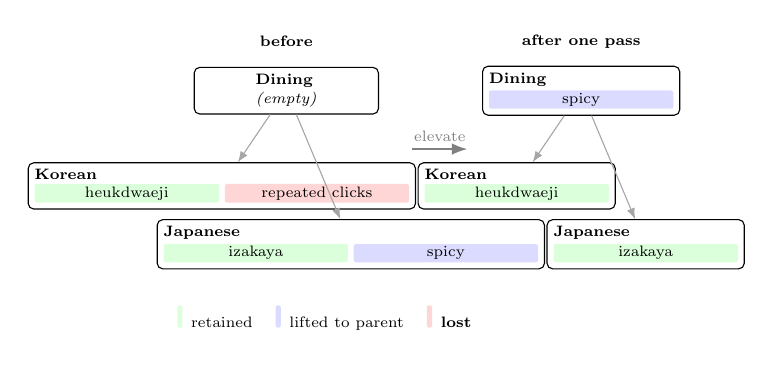
\begin{tikzpicture}[
  scale=0.78, transform shape,
  font=\scriptsize,
  note/.style={draw, rounded corners=2pt, align=left, inner sep=3pt, minimum width=30mm},
  kw/.style={rounded corners=1pt, inner sep=1.2pt, font=\scriptsize},
  keep/.style={kw, fill=green!14},
  lift/.style={kw, fill=blue!14},
  lost/.style={kw, fill=red!16},
  arr/.style={-{Latex[length=1.4mm]}, gray!70},
]
%% before
\node[note] (pb) at (0,1.55) {\textbf{Dining}\\[1pt] \textit{(empty)}};
\node[note] (kb) at (-1.05,0) {\textbf{Korean}\\[1pt] \tikz\node[keep]{heukdwaeji};\ \tikz\node[lost]{repeated clicks};};
\node[note] (jb) at (1.05,-0.95) {\textbf{Japanese}\\[1pt] \tikz\node[keep]{izakaya};\ \tikz\node[lift]{spicy};};
\draw[arr] (pb) -- (kb); \draw[arr] (pb) -- (jb);
\node[font=\scriptsize\bfseries] at (0,2.35) {before};

%% after
\begin{scope}[xshift=48mm]
\node[note] (pa) at (0,1.55) {\textbf{Dining}\\[1pt] \tikz\node[lift]{spicy};};
\node[note] (ka) at (-1.05,0) {\textbf{Korean}\\[1pt] \tikz\node[keep]{heukdwaeji};};
\node[note] (ja) at (1.05,-0.95) {\textbf{Japanese}\\[1pt] \tikz\node[keep]{izakaya};};
\draw[arr] (pa) -- (ka); \draw[arr] (pa) -- (ja);
\node[font=\scriptsize\bfseries] at (0,2.35) {after one pass};
\end{scope}

\draw[-{Latex[length=2mm]}, thick, gray] (2.05,0.6) -- (2.95,0.6)
  node[midway, above, font=\scriptsize] {elevate};

%% legend
\node[anchor=west, font=\scriptsize] at (-1.9,-2.15)
  {\tikz\node[keep]{\strut};\, retained \quad
   \tikz\node[lift]{\strut};\, lifted to parent \quad
   \tikz\node[lost]{\strut};\, \textbf{lost}};
\end{tikzpicture}
\caption{The instrument. Every keyword at a non-root note lands in exactly one bucket after a pass: still on its own note (\emph{retained}), moved to the parent (\emph{lifted}, the intended behaviour), or on neither (\emph{lost}). Here ``spicy'' is correctly promoted and ``heukdwaeji'' kept, but ``repeated clicks'' --- the evidence supporting a claim --- is deleted without appearing anywhere.}
\Description{A two-panel tree diagram. Before consolidation, a Dining parent node is empty and has two child notes, Korean and Japanese, each holding keywords. After one elevation pass, the shared keyword has moved to the parent, one concrete keyword remains at each child, and one keyword has disappeared entirely, illustrating the three outcome categories retained, lifted, and lost.}
\label{fig:instrument}
\end{figure}

Two clauses do the work, both from an audit of our own earlier measurements. The prose clause: a keyword can leave the \texttt{keywords} field while the concept survives in the summary beside it, and \(19.2\%\) of keywords missing from both keyword fields do still appear verbatim in the surrounding prose, so requiring absence from the text makes \(\mathrm{LossRate}\) conservative on that axis rather than a keyword-churn count. The relocation clause: merging writes a unified note at a new path, so a rule inspecting only the original path and its parent scores relocated content as deleted --- which inflates merging's apparent contribution by an order of magnitude (Section~\ref{sec:merge}). We therefore scope survival to the parent, the original note, and paths the pass \emph{created} beneath that parent: provably inert wherever nothing moved, and verified to be where merges land, since every new path in our full-backward runs appeared under a parent that had lost a child (\(340/340\) and \(338/338\)).

We do \emph{not} credit survival by substring (\emph{jiu-jitsu} inside \emph{Brazilian jiu-jitsu}), which would apply to \(20.9\%\) of losses. Korean morphology cuts the other way, but normalizing josa and verb endings on both sides moves \(\mathrm{LossRate}\) by at most \(0.003\).

We report \(\mathrm{LossRate} = |\text{lost}| / (|\text{retained}| + |\text{lifted}| + |\text{lost}|)\), aggregated as the post-stratified mean of per-user rates (paired differences are unweighted means).


\subsection{Data}
\label{sec:data}

We work from the production build output of a large-scale Korean map service, which writes one row per (user, note) for every user whose behaviour changed that day. The service processes \(99{,}993\)--\(99{,}999\) users daily (a top-\(100\text{K}\) cap) and \(1{,}977{,}833\) distinct users over the 36-day window we retain.

\paragraph{Stratification.} Elevation can only promote what siblings share, so we stratify by \emph{headroom}, the saving Eq.~\eqref{eq:elevation-savings} predicts of a lossless elevation: \(\sum_{i \in I}(k_i-1)\) over a user's tree. Over one full day of production memory it is small, and \(17.6\%\) of users sit at zero, so uniform sampling would over-weight users on whom elevation can do almost nothing. Four strata follow: \textbf{zero} (\(0\)), \textbf{low} (\(1\)--\(3\)), \textbf{mid} (\(4\)--\(9\)), \textbf{high} (\(\geq 10\)). The \textbf{zero} stratum is the control behind this paper's sharpest result: these users have siblings but no shared keyword, so a correct elevation leaves them untouched.

\paragraph{Frozen datasets.} Two snapshots, each \(500\) users per split with \(125\) per stratum, fixed seed, pinned by content hash. \textsc{Mech} (2026-08-17, \(7{,}924\) notes) carries the loss measurements; \textsc{Eval} (2026-07-15, \(7{,}275\) notes) adds a held-out MCQ target (Section~\ref{sec:mcq}). Both reserve a disjoint test half of equal size and stratum balance. Loss numbers in Sections~\ref{sec:loss}--\ref{sec:persona} and the accuracy comparison of Section~\ref{sec:mcq} are on the development half; the two experiments on \(977\) users (Sections~\ref{sec:guard} and~\ref{sec:delivery}) pool both halves, a pre-registered design that is not a fresh sample. The test half was opened once for the comparisons declared in advance. One qualification applies: after that opening we audited our instrument, corrected two defects (the prose and relocation clauses of Section~\ref{sec:loss}), and recomputed \emph{both} halves under the corrected rule. The correction was motivated by the mechanics of merging, not by anything in the held-out results, and replays stored snapshots deterministically --- but it is a post-hoc change, and we name it rather than let ``opened once'' carry more weight than it can. Because strata are over-sampled relative to the population, every aggregate we report is post-stratified back to the population proportions recorded in the snapshot manifest.

\paragraph{Backbones and isolation.} \texttt{gemma-4-31b-it} unless stated; \texttt{qwen3-\allowbreak 30b-\allowbreak a3b-\allowbreak instruct} (deployed) and \texttt{qwen3-\allowbreak 235b-\allowbreak a22b-\allowbreak instruct}~\cite{qwen3} for the model comparison, all served in-house through the same vLLM~\cite{vllm} gateway. The client exposes no seed, so repeated runs measure sampling variance rather than reproducing a draw; three repeats spread \(\pm 0.003\), a thirtieth of the headline effects below, so single runs are reported elsewhere. Elevation is run alone unless stated: merging renames paths, which breaks keyword tracking, and pruning cannot fire at these node ages (8--34 days against a 120-day threshold). Section~\ref{sec:merge} adds merging back deliberately. Every variant starts from a deep copy of the same tree, so comparisons are paired per user, and the runner aborts if the arms' pre-consolidation keyword totals ever differ.


\subsection{Consolidation deletes, including where there is nothing to compress}

\begin{figure}[t]
\centering
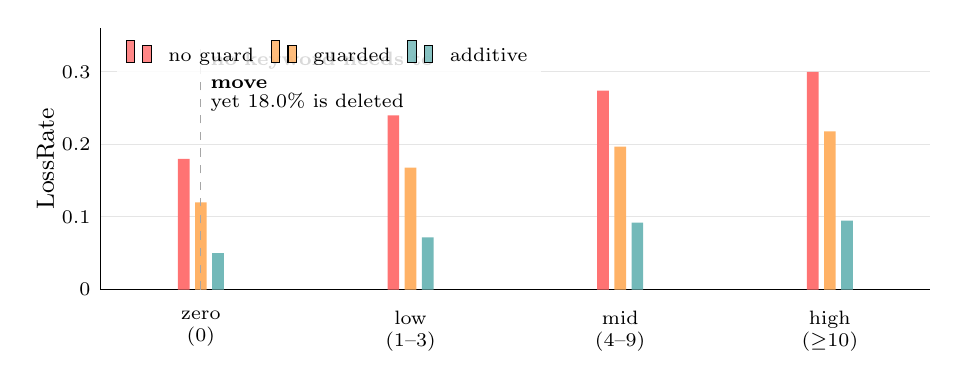
\begin{tikzpicture}
\begin{axis}[
  width=\linewidth, height=4.9cm,
  ybar, bar width=4.2pt,
  enlarge x limits=0.16,
  ymin=0, ymax=0.36,
  ylabel={LossRate}, ylabel style={font=\small, yshift=-4pt},
  symbolic x coords={zero,low,mid,high},
  xtick=data,
  xticklabels={{zero\\(0)},{low\\(1--3)},{mid\\(4--9)},{high\\($\geq$10)}},
  xticklabel style={align=center, font=\scriptsize},
  yticklabel style={font=\scriptsize},
  legend style={font=\scriptsize, at={(0.02,0.98)}, anchor=north west,
                draw=none, fill=white, fill opacity=0.85, text opacity=1,
                legend columns=3, column sep=4pt},
  tick style={draw=none},
  ymajorgrids, grid style={gray!20},
  axis lines*=left,
]
\addplot[fill=red!55, draw=none] coordinates {(zero,0.180) (low,0.240) (mid,0.274) (high,0.300)};
\addplot[fill=orange!60, draw=none] coordinates {(zero,0.120) (low,0.168) (mid,0.197) (high,0.218)};
\addplot[fill=teal!55, draw=none] coordinates {(zero,0.050) (low,0.072) (mid,0.092) (high,0.095)};
\legend{no guard, guarded, additive}
\draw[dashed, gray!70] (axis cs:zero,0) -- (axis cs:zero,0.34);
\node[font=\scriptsize, anchor=north west, align=left, text width=3.4cm]
  at (axis cs:zero,0.34) {\textbf{no keyword needs to move}\\[-1pt] yet \(18.0\%\) is deleted};
\end{axis}
\end{tikzpicture}
\caption{Loss rises with headroom --- the saving Eq.~\eqref{eq:elevation-savings} predicts a lossless elevation would achieve --- for every variant (\texttt{gemma-4-31b}, 500 production trees, 125 users per stratum). The leftmost group is the control: these users' siblings share no keyword, so nothing needs to move, and \(18.0\%\) is deleted anyway. The guard's benefit grows with headroom too, \(-0.059\) at zero to \(-0.081\) at high. \textsc{additive} never rewrites children, so its loss is confined to Level-2 notes acting as parents and it is shown for shape rather than as a like-for-like comparison.}
\Description{Grouped bar chart of loss rate against headroom stratum for three elevation variants. Loss increases monotonically from the zero stratum to the high stratum for every variant, and the zero stratum, where no keyword is shared between siblings, still shows substantial loss.}
\label{fig:dose}
\end{figure}

Figure~\ref{fig:dose} reports the instrument on 500 production trees. Weighted to the population, unguarded elevation loses \(0.253\) of all child keywords under the conservative definition, the deployed guard \(0.181\) (\(\Delta = -0.071\)). Two features matter more than that headline.

\paragraph{The zero stratum loses \(18.0\%\).} These users' siblings share no keyword, so Eq.~\eqref{eq:elevation-savings} predicts a keyword-level saving of exactly zero. Nearly a fifth of their concrete tokens disappear anyway. We are careful about what that shows: the agent reads whole summaries, not keyword lists, and zero-stratum siblings still share summary vocabulary (\(9.1\) tokens per parent group against \(19.6\) in the high stratum), so promoting a shared \emph{theme} is legitimate and the pass need not have been a no-op. The narrower claim still damages: a faithful rewrite promoting a shared theme has no reason to delete a child's \emph{unique} keywords, and those are exactly what disappears. The loss looks collateral to the rewrite rather than a product of compression. The control removes lexical headroom only and we have no rewrite-only baseline, so this names the likeliest cause rather than isolating it.

\paragraph{Loss scales with headroom, and lifting is rare.} Loss rises monotonically with the amount genuinely shared (\(0.180 \to 0.300\)), and so does the guard's benefit (\(-0.059 \to -0.081\)) Meanwhile keywords classified as \emph{lifted} account for at most \(6.2\%\) of the total in any variant. Elevation as executed is overwhelmingly a delete rather than a move: the parent receives an abstraction and the child's concrete token is discarded, not relocated.

\paragraph{Loss versus compression.} Between the two variants that rewrite children (summary text \(-39.4\%\) destructive, \(-5.8\%\) additive), guarded elevation retains \(84\%\) of destructive's compression while cutting loss by \(28\%\).

\subsection{The magnitude belongs to the backbone}
\label{sec:models}
Identical prompts over identical trees on three backbones: the operation does not behave the same way twice (Figure~\ref{fig:backbones}). Gemma compresses hard and loses hard (LossRate \(0.255\) unguarded in these runs, keywords \(-34.0\%\)); the Qwen models lose far less (\(0.102\) on the 235B, \(0.063\) on the 30B), the 235B barely compresses (\(-11.9\%\)) and the deployed 30B \emph{inflates} (\(+5.0\%\)) --- it returns more keywords than it was given. The guard follows suit: decisive on Gemma (\(\Delta = -0.073\), \(d = -0.70\); \(-0.071\) in the main runs), inert on the 235B (\(+0.002\)), and on the 30B a \emph{significant increase} in loss (\(+0.006\), 95\% CI \([+0.001, +0.011]\), \(p = 0.016\)). The effect is small; its sign is the point. A mitigation validated on one backbone can be harmful on another, while the failure mode itself is universal in direction, since all three models lose keywords in the zero stratum.

\begin{figure}[t]
  \centering
  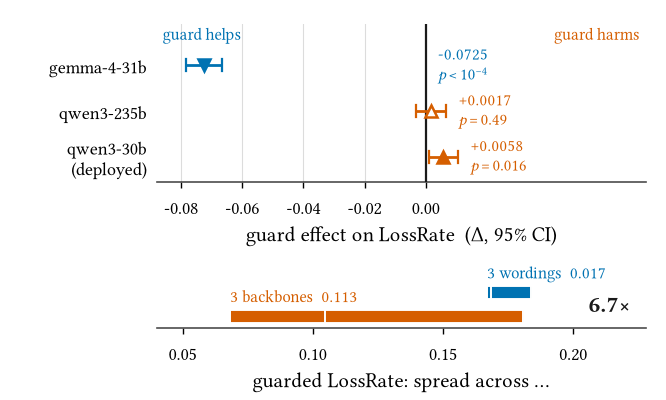
\includegraphics[width=0.92\linewidth]{figures/backbones.png}
  \Description{Top: a forest plot of the guard's effect on loss rate for three backbones. The guard lowers loss on gemma-4-31b, has no measurable effect on qwen3-235b, and slightly raises loss on the deployed qwen3-30b. Bottom: guarded loss rate varies by 0.113 across the three backbones but only 0.017 across three wordings of the prompt, a factor of 6.7.}
  \caption{The guard's effect on LossRate by backbone (\(\Delta\), 95\% CI; blue helps, orange harms). Below, the spread of guarded LossRate across the three backbones (\(0.113\)) against the spread across three wordings of the prompt on gemma (\(0.017\)), a factor of \(6.7\).}
  \label{fig:backbones}
\end{figure}

\paragraph{The backbone, not the phrasing.} Those runs share one wording. Two paraphrases of the elevation instruction --- every proposition preserved, only voice, clause order, list format and terminology changed --- on gemma over 150 users move guarded \(\mathrm{LossRate}\) across \(0.167\)--\(0.184\): a spread of \(0.017\) against \(0.113\) across the backbones (\(0.182\), \(0.104\), \(0.069\)), a factor of \(6.7\). The guard survives rephrasing, cutting loss by \(0.082\), \(0.068\) and \(0.054\) under the three wordings, each at \(p < 10^{-4}\). Phrasing is not nothing (one paraphrase costs \(+0.015\), the other is indistinguishable) but is several times smaller than the choice of model.

\subsection{The deployed guard protects the wrong tokens}
\label{sec:guard}
The guard shipped in production names place names, store names and brands. Typing every keyword and comparing its share of losses against its share of survivors (Figure~\ref{fig:tokens}) asks whether those are what disappears. They are not. Place names (ratio \(0.58\)) and brands (\(0.76\)) are \emph{under}-represented among losses, so the deployed guard is defending tokens that were never in danger \emph{here} --- Section~\ref{sec:delivery} finds them destroyed one stage later instead. What is lost in bulk is category vocabulary (\emph{grilled meat}, \emph{gukbap}, \emph{Chinese}, \emph{Korean}) and, at \(2.36\times\) its base rate, the behavioural evidence that grounds a claim (\emph{repeated clicks}, \(184\) occurrences). That second group is the more damaging: the extraction prompt requires every persona claim to cite click evidence, and elevation removes those citations at over twice their base rate, leaving assertions whose support is silently gone.

\begin{figure}[t]
  \centering
  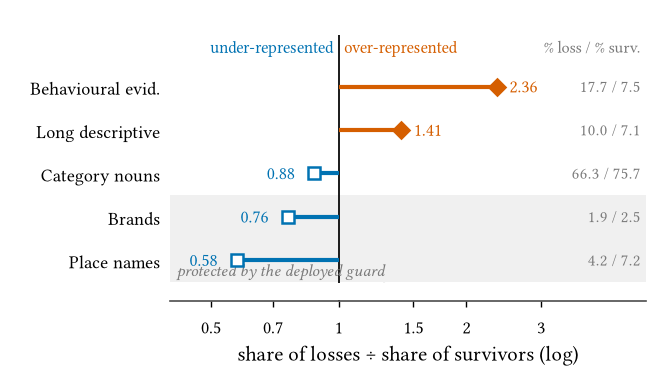
\includegraphics[width=0.92\linewidth]{figures/tokens.png}
  \Description{A lollipop chart on a log axis of the share of losses divided by the share of survivors for five token types. Behavioural evidence is over-represented among losses at 2.36 times and long descriptive phrases at 1.41. Category nouns at 0.88, brands at 0.76 and place names at 0.58 are under-represented. Place names and brands are the tokens the deployed guard protects.}
  \caption{What unguarded elevation removes, by token type (\texttt{gemma-4-31b}, 500 production trees): share of all lost keywords divided by share of surviving keywords. Above \(1\) a type is over-represented among losses. Place names and brands, which the deployed guard protects, survive above their base rate; behavioural evidence (most often \emph{repeated clicks}, \(184\) occurrences) is lost at \(2.36\times\) its base rate.}
  \label{fig:tokens}
\end{figure}

\paragraph{A guard derived from the measurement.} We rewrote the instruction around what the data says is at risk --- category, cuisine and business-type nouns, place and brand names, behavioural evidence --- disallowing generic superclasses such as ``diverse food''. The structural operation is unchanged; the cost is one prompt line (wording in Appendix~\ref{app:guard}). LossRate falls from \(0.253\) to \(0.181\) (deployed) to \(0.160\) (v2) (Table~\ref{tab:guard}), all three paired differences surviving Holm correction at \(p < 0.0001\); v2 cuts a further \(11\%\) of the deployed guard's loss while compressing slightly less --- the expected direction, since the tokens it saves are tokens that would otherwise have been deleted.

\begin{table*}[t]
\caption{Guard wording on the development half (500 users, \texttt{gemma-4-31b}) and the reserved half. Paired differences are unweighted per-user means with 95\% bootstrap CIs; \(d\) is Cohen's \(d\); LossRate is post-stratified.}
\label{tab:guard}
\small
\setlength{\tabcolsep}{5pt}
\begin{tabular}{lcccccccc}
\toprule
 & \multicolumn{4}{c}{development half} & \multicolumn{3}{c}{reserved half} \\
\cmidrule(lr){2-5}\cmidrule(lr){6-8}
 & LossRate & summary text & \(\Delta\) vs.\ no guard [95\% CI] & \(d\) & LossRate & \(\Delta\) vs.\ no guard & \(d\) \\
\midrule
no guard         & \(0.253\) & \(-39.2\%\) & --- & --- & \(0.251\) & --- & --- \\
deployed guard   & \(0.181\) & \(-32.9\%\) & \(-0.071\) \([-0.077,-0.066]\) & \(-0.68\) & \(0.178\) & \(-0.071\) & \(-0.68\) \\
\textsc{guard-v2} & \(0.160\) & \(-29.2\%\) & \(-0.092\) \([-0.098,-0.086]\) & \(-0.88\) & \(0.160\) & \(-0.089\) & \(-0.86\) \\
v2 vs.\ deployed & --- & --- & \(-0.021\) \([-0.024,-0.016]\) & \(-0.22\) & --- & \(-0.018\) \([-0.022,-0.014]\) & \(-0.19\) \\
\bottomrule
\end{tabular}
\end{table*}

\paragraph{We tried to price the difference, and could not.} Everything above is observational --- it says which tokens leave, not what their leaving costs. So we deleted tokens ourselves, which no prompt can make an agent do selectively. On 977 users we built five versions of each real tree: untouched, and four with tokens removed at random, from what the guard protects, from what it leaves exposed, and the entire exposed pool. The three middle arms delete an \emph{identical} count per user, so a difference between them is attributable to which tokens went rather than how many.  The design was registered in advance.

Nothing moved, and the exact zero turned out to be structural. The registered contrast was \(0.0000\) (95\% CI \([-0.021,+0.021]\)) because the persona is generated from the notes' \texttt{summary} text alone --- we verified against the deployed agent that \texttt{keywords} never reaches the generator, so a deletion confined to that field cannot reach the artifact the probe consumes. Re-running it striking the same victims from the surrounding prose, as real consolidation does, does reach: no two arms share a persona and \(26.4\%\) of users change their answer, for a median \(367\) characters removed. Accuracy still does not move (\(+0.011\), 95\% CI \([-0.015,+0.038]\), \(p = 0.43\)). That is a fact about the probe rather than the memory (Section~\ref{sec:mcq}).

\subsection{Merging relocates; it does not delete}
\label{sec:merge}
Running the full backward pass isolates what merging adds --- and exposes an artifact of the kind an instrument of this shape invites (Table~\ref{tab:merge}). Merging is the only backward operation that \emph{moves} a note: it deletes its sources and writes a unified note under a different path, so an instrument looking only at a keyword's own path and its parent scores everything a merge carried as deleted, and the full pass appears to make merging responsible for \(23\%\) and \(33\%\) of the total. It is not: of the keywords that rule calls lost, \(38.6\%\) unguarded and \(48.6\%\) guarded are still present elsewhere in the same tree. Under the relocation-aware scope of Section~\ref{sec:loss} merging adds almost nothing, while still removing \(5.2\%\) of notes, its intended effect. \textbf{Merging relocates; it does not delete.} Consolidation loss belongs to elevation, which says where a guard is worth building. It also generalizes: any keyword-level tracker will mis-attribute deletion to whichever operation renames things, here by an order of magnitude.

\begin{table}[t]
\caption{What merging adds, by instrument (\texttt{gemma-4-31b}, 500 users). Elevation alone is the baseline; the same-path rule counts a moved keyword as lost.}
\label{tab:merge}
\small
\begin{tabular}{lcc}
\toprule
 & unguarded & guarded \\
\midrule
elevation alone, LossRate & \(0.253\) & \(0.181\) \\
full pass, same-path rule & \(0.328\) (\(+0.075\)) & \(0.268\) (\(+0.088\)) \\
\quad share of that total & \(23\%\) & \(33\%\) \\
full pass, relocation-aware & \(+0.001\) (\(p=0.75\)) & \(+0.007\) (\(p=0.003\)) \\
\quad 95\% CI & --- & \([+0.002,+0.012]\) \\
lost keywords still in the tree & \(38.6\%\) & \(48.6\%\) \\
\bottomrule
\end{tabular}
\end{table}

\subsection{The loss reaches what the ranker reads}
\label{sec:persona}
A downstream ranker never sees the memory; it sees a persona synthesized from a few selected paths, so loss inside the tree matters only if it survives that step. We generated a persona from each tree before and after consolidation and asked how many of the removed keywords also vanished from it (\(n=200\)). Propagation is \(0.765\) without a guard, \(0.711\) with the deployed one, and \(0.713\) with v2 --- above \(70\%\) in every arm, and flat across the two guarded ones. The guard does not make the persona more robust to loss; it reduces how much is lost in the first place, which carries through to \(21\%\) fewer keywords missing from the final persona (\(372 \to 295\)).

\paragraph{The paths do not move.} Path selection is itself an LLM call, so a keyword could vanish because a different subtree was read. Recording the chosen paths rules that out: mean Jaccard between pre- and post-consolidation path sets is \(0.90\)--\(0.92\), the sets are \emph{identical} for \(67.5\%\)--\(72.5\%\) of users, and restricting to those users moves propagation by at most \(0.021\). We have no propagation rate for retained keywords, and Section~\ref{sec:delivery} finds the persona discarding much that the tree keeps, so this shows that the loss is not recovered downstream, not that consolidation causes it.

\subsection{The delivery path costs more than consolidation does}
\label{sec:delivery}
The tree is not what the ranker reads: between the two sits a delivery path --- select a few paths, synthesise a persona --- which is itself two compression steps we had never measured. We measured them on the same \(977\) users and held-out questions, varying only what the model is given (Table~\ref{tab:delivery}); instruction, question and option ordering are byte-identical across arms.

\begin{table}[t]
\caption{What the model is given and the MCQ accuracy it reaches (\(977\) users, both halves pooled; the floor is on \(471\) development-half users). Gains are paired differences with 95\% CIs; all survive Holm at \(p<10^{-4}\).}
\label{tab:delivery}
\small
\resizebox{\columnwidth}{!}{\begin{tabular}{llcc} \toprule arm & given to the model & accuracy & gain over deployed \\ \midrule no memory & empty persona & \(0.226\) & --- \\ \textbf{deployed} & select paths, synthesise & \(0.459\) & --- \\ flat + synthesis & all notes, flattened, synthesised & \(0.575\) & \(+0.117\) \([+0.083,+0.149]\) \\ raw notes & all summaries, no synthesis & \(0.649\) & \(+0.190\) \([+0.156,+0.226]\) \\ \bottomrule \end{tabular}}
\end{table}

Both steps are negative: flattening the tree is worth \(+0.117\), and dropping synthesis as well a further \(+0.074\) (\([+0.047,+0.100]\)). On the \(471\) users for whom the floor was measured, the deployed persona earns \(+0.248\) over it and the delivery path forgoes \(+0.184\) more: \(74\%\) of the deployed memory's own gain, \(43\%\) of what the raw notes would earn.

\paragraph{Where it goes.} Place names survive consolidation well (Section~\ref{sec:guard}) but not delivery: the median user's notes carry six distinct place names and the median retention into the persona is \(0.00\); \(63\%\) of users keep none. The guard protects tokens through the tree and the next stage discards them anyway.

\paragraph{One confound, measured.} Distractors are matched on category and review count but not location, so geography is a cue available to the raw-notes arm and not the deployed one. Splitting on whether any option title carries an area name from the user's notes, the gap is \(+0.285\) where it does (\(n = 172\)) and \(+0.170\) where it does not (\(n = 805\)), both at \(p < 10^{-4}\). The confound inflates the effect; it does not produce it.

\subsection{Downstream accuracy: ordered but not resolved}
\label{sec:mcq}
\paragraph{Held-out task.} To avoid leakage we take an older snapshot (2026-07-15) and hold out everything after: the target is each user's first qualified review in 2026-07-16..08-20, against three same-category distractors matched on review count. Appendix~\ref{app:mcq} gives the construction and the filtering it forced.

Accuracy orders exactly inversely to LossRate --- \(0.452\) destructive, \(0.466\) guarded, \(0.472\) v2, \(0.484\) with no consolidation --- but no pairwise difference against the no-guard arm is significant (\(p = 0.46\), \(0.30\), \(0.13\); widest CI \([-0.008, +0.072]\)), and per-user correlation between LossRate and answering correctly is \(\approx 0\) in every arm (\(|r| \leq 0.05\)). 

A null is only interpretable against a floor: a \textsc{no memory} arm scores \(0.226\), no better than guessing, and the whole consolidation span is an eighth of what memory is worth, so sample size is the obvious explanation. Two results rule it out. Section~\ref{sec:guard}'s intervention deleted enough to change \(26.4\%\) of the answers and left accuracy untouched (\(+0.011\), \(p = 0.43\)); Section~\ref{sec:delivery} moves the same probe by \(+0.190\) by changing only how the memory is delivered. The probe's resolution is sharply shaped rather than absent: it reads \emph{how} a memory reaches the model and not \emph{which tokens} the tree holds. What the data do support is narrower: guarded consolidation is indistinguishable from not consolidating (\(\Delta = 0.018\), \(p = 0.39\)) while removing a third of the memory's text.

\subsection{Held-out confirmation}
\label{sec:heldout}
Every loss comparison above was developed on one half of each snapshot; the reserved half was opened once, with model, prompts and analysis fixed, then recomputed once when we corrected the instrument (Section~\ref{sec:data}). This matters most for \textsc{guard-v2}, whose wording came from the development half's loss profile.

The loss measurements replicate to within \(0.003\) (Table~\ref{tab:guard}, right), all three paired differences remain significant at \(p < 0.0001\) after Holm correction, and the effect sizes are essentially unchanged. The zero-headroom control holds, at \(18.2\%\) against \(16.9\%\) (\(18.0\%\) in Figure~\ref{fig:dose}) --- the widest gap, and the one place the reserved half is kinder. \textsc{guard-v2} retains its advantage over the deployed guard, slightly attenuated (\(-0.021\) to \(-0.018\)) --- the direction expected when a rule tuned on one sample meets another.

The accuracy null replicates, instructively: held-out accuracy runs \(0.468\), \(0.466\), \(0.448\), \(0.436\) with nothing significant, and the ordering that matched LossRate exactly on the development half breaks. The loss is real and reproducible; this task cannot see it.



%% ============================================================
%% DEPLOYMENT
%% ============================================================
\section{Deployment}
\label{sec:governance}

\paragraph{Scale and cost.} Forward aggregation costs about ten LLM calls per user per update (Eq.~\eqref{eq:forward-cost}, \(N \approx 8.0\)) and elevation adds \(2.99\). The dominant cost is implicit extraction at 73K input tokens per user; clustering similar inputs before the LLM~\cite{personax} and distilling into a smaller model~\cite{personamem-v2} are the plausible reductions.

\paragraph{Consolidation is not free, and is not running.} Over 497 consecutive update pairs from 429 users (median gap 17 days), notes per user grow \(16.4\%\), keywords \(29.5\%\) and summary text \(24.0\%\) per update, with \(472/497\) pairs increasing. Our deployment has run consolidation once, over 35 users in a test namespace: \texttt{last\_cleaned\_at} is null for every user in current production output. Those growth figures therefore describe the unconsolidated regime rather than a counterfactual.

\paragraph{Sensitive information.} Three mechanisms, none described in our earlier writeup. At routing time, paths whose Level-2 segment matches a blocked category (medical, health, hospital, religion, politics) or that contain a blocked token anywhere are dropped before any note is written --- why the deployed taxonomy has ten domains rather than the eleven specified. A filtering job separately runs LLM-based detection over every summary, masks the spans it flags, and records a boolean audit column. One inconsistency remains: the implicit-extraction prompt still lists a medical domain, so such content is extracted and only then discarded at routing. The third mechanism deleted a field rather than filtering one: a security review conditioned the memory API's clearance on removing \texttt{user\_info}, which was withdrawn from the API response, then the prompts and pipeline schema, then the stored Iceberg column and serving index. An external review can retire a field after deployment, and a consolidation policy that assumes a stable schema will not age well.

\paragraph{What the code enforces.} Depth \(\leq 3\) and root-exclusive demographics are requested in prompts and not checked in code --- though zero Level-4 paths appeared across all 24 elevation runs and both full-backward runs, so the prompt-level bound holds in practice. Merging takes the maximum update count among its sources rather than the sum, which keeps repeated consolidation a fixed point.

\paragraph{What we can and cannot release.} The memory trees are production user data and cannot leave the company, so these measurements are not externally reproducible in the strict sense. The instrument is portable: a few hundred lines with no dependency on our data, applicable to any memory whose notes carry an explicit term field. The agent under measurement reaches us as compiled bytecode, so merge destinations are measured, not argued from source. Per-run artifacts are pinned by content hash, and the mismatches our own audit surfaced are corrected in this version.
\section{Conclusion and Future Work}
\label{sec:limitations}

Hierarchical memory systems consolidate themselves, and the step has until now been assessed only by what it saves and what survives downstream. Following individual keywords through it on deployed memory shows it is not doing what its formalization says. A quarter of child keywords vanish from the note and its prose alike, deletion far outnumbers relocation, and users whose siblings share no keyword --- for whom nothing needs to move --- still lose \(18\%\) of their concrete tokens; over \(70\%\) of removed keywords are also missing from the persona the ranker reads. 

Three consequences follow. The deployed guard protected place names and brands, never at risk, while category vocabulary and the behavioural evidence behind each claim (\(2.4\times\) its base rate) disappeared; a guard rewritten from the measured profile removes a further \(11\%\) of the deployed guard's loss for one prompt line. Sibling merging relocates notes rather than deleting them, and an instrument that does not follow the relocation reports that as roughly a quarter of all loss. And none of it transfers between backbones: a prompt validated on one model is evidence about that model only, and can be worse than nothing elsewhere.

We could not close the chain to accuracy, and we now know why. Deleting the exposed pool from the notes \emph{and} from the prose the persona is written from changes \(26.4\%\) of the answers and still leaves accuracy untouched (\(+0.011\), \(p = 0.43\)). A four-way choice over same-category venues is insensitive to keyword-level memory content, so more users would not have rescued it. The same probe is not insensitive to everything. Holding the memory fixed and varying only its delivery --- selecting paths, then synthesizing a persona --- costs \(+0.190\) accuracy against handing over the raw notes, three quarters of the gain the deployed memory delivers over an empty persona. The step we instrumented is the cheaper of the two compressions in the pipeline, by roughly a factor of six. Three limitations remain: consolidation has run once over 35 users, so our growth rates describe the unconsolidated regime rather than a controlled comparison; guard-v2 was derived and tested on one backbone; and the prompts and taxonomy are Korean --- the failure mode is unlikely to be language-specific, but the guard's wording certainly is.

What we would ask of anyone building such a system is the thing we did not do while operating ours: look at the maintenance step directly. Instrumenting it needs no labels and no downstream task, and a few hundred lines of it found a guard defending tokens that were never at risk, an operation we had blamed for roughly a quarter of the loss that does not delete at all, and a prompt that helps one backbone while harming the one we shipped. And the one thing that did move accuracy was the step we never thought to question.

%% ============================================================
%% APPENDIX
%% ============================================================
\clearpage
\appendix

\section{Motivating example}
\label{app:motivation}

\begin{figure}[t]
  \centering
  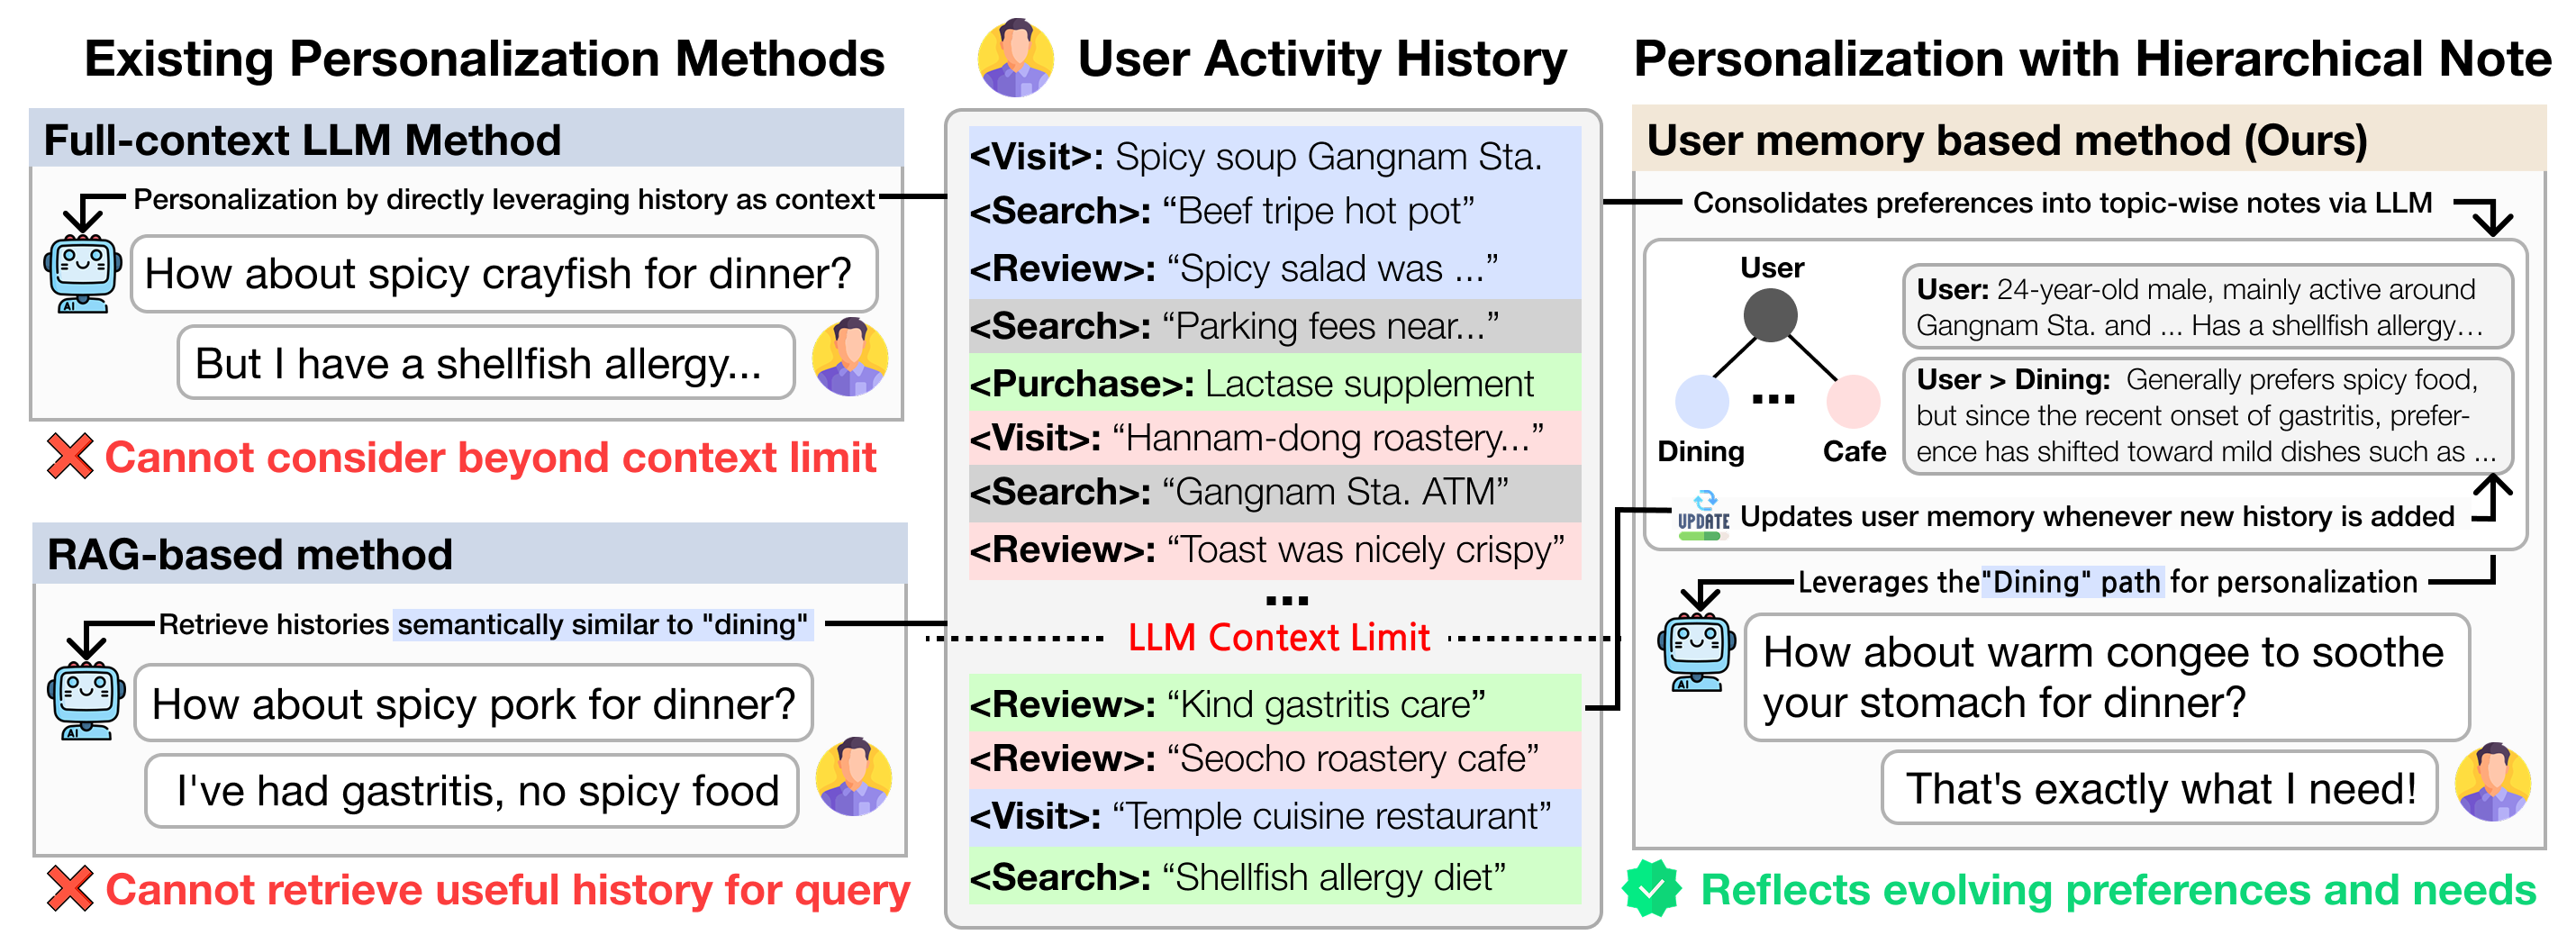
\includegraphics[width=\linewidth]{figures/intro_memory.png}
  \Description{Three-panel comparison of personalization on a dining query for a user whose preferences shifted from spicy to mild after a gastritis episode: a full-context LLM and a RAG baseline both recommend spicy dishes by missing the gastritis signal, while a hierarchical-note memory consolidates activities into topic-wise notes and recommends warm congee. The consolidation step shown in the third panel is the operation the paper goes on to measure.}
  \caption{Why the memory has to contract, and what it risks. An illustrative user's preferences have evolved (spicy $\to$ mild after gastritis; the deployed system filters health content, Section~\ref{sec:governance}). \textit{Left:} a full-context LLM cannot reason past its context limit, and RAG retrieves entries similar to ``dining'' while missing the gastritis signal, so both recommend spicy dishes. \textit{Middle:} the raw history exceeds the context window and the decisive evidence is scattered across sessions --- the pressure that motivates a compact, structured memory. \textit{Right:} hierarchical notes consolidate that history and surface the evolved preference. The consolidation step this figure takes for granted is what the rest of the paper measures: the same operation that keeps ``mild, gastritis'' usable can also delete it.}
  \label{fig:overview}
\end{figure}

\section{Memory schema detail}
\label{app:schema}

\begin{figure}[t]
  \centering
  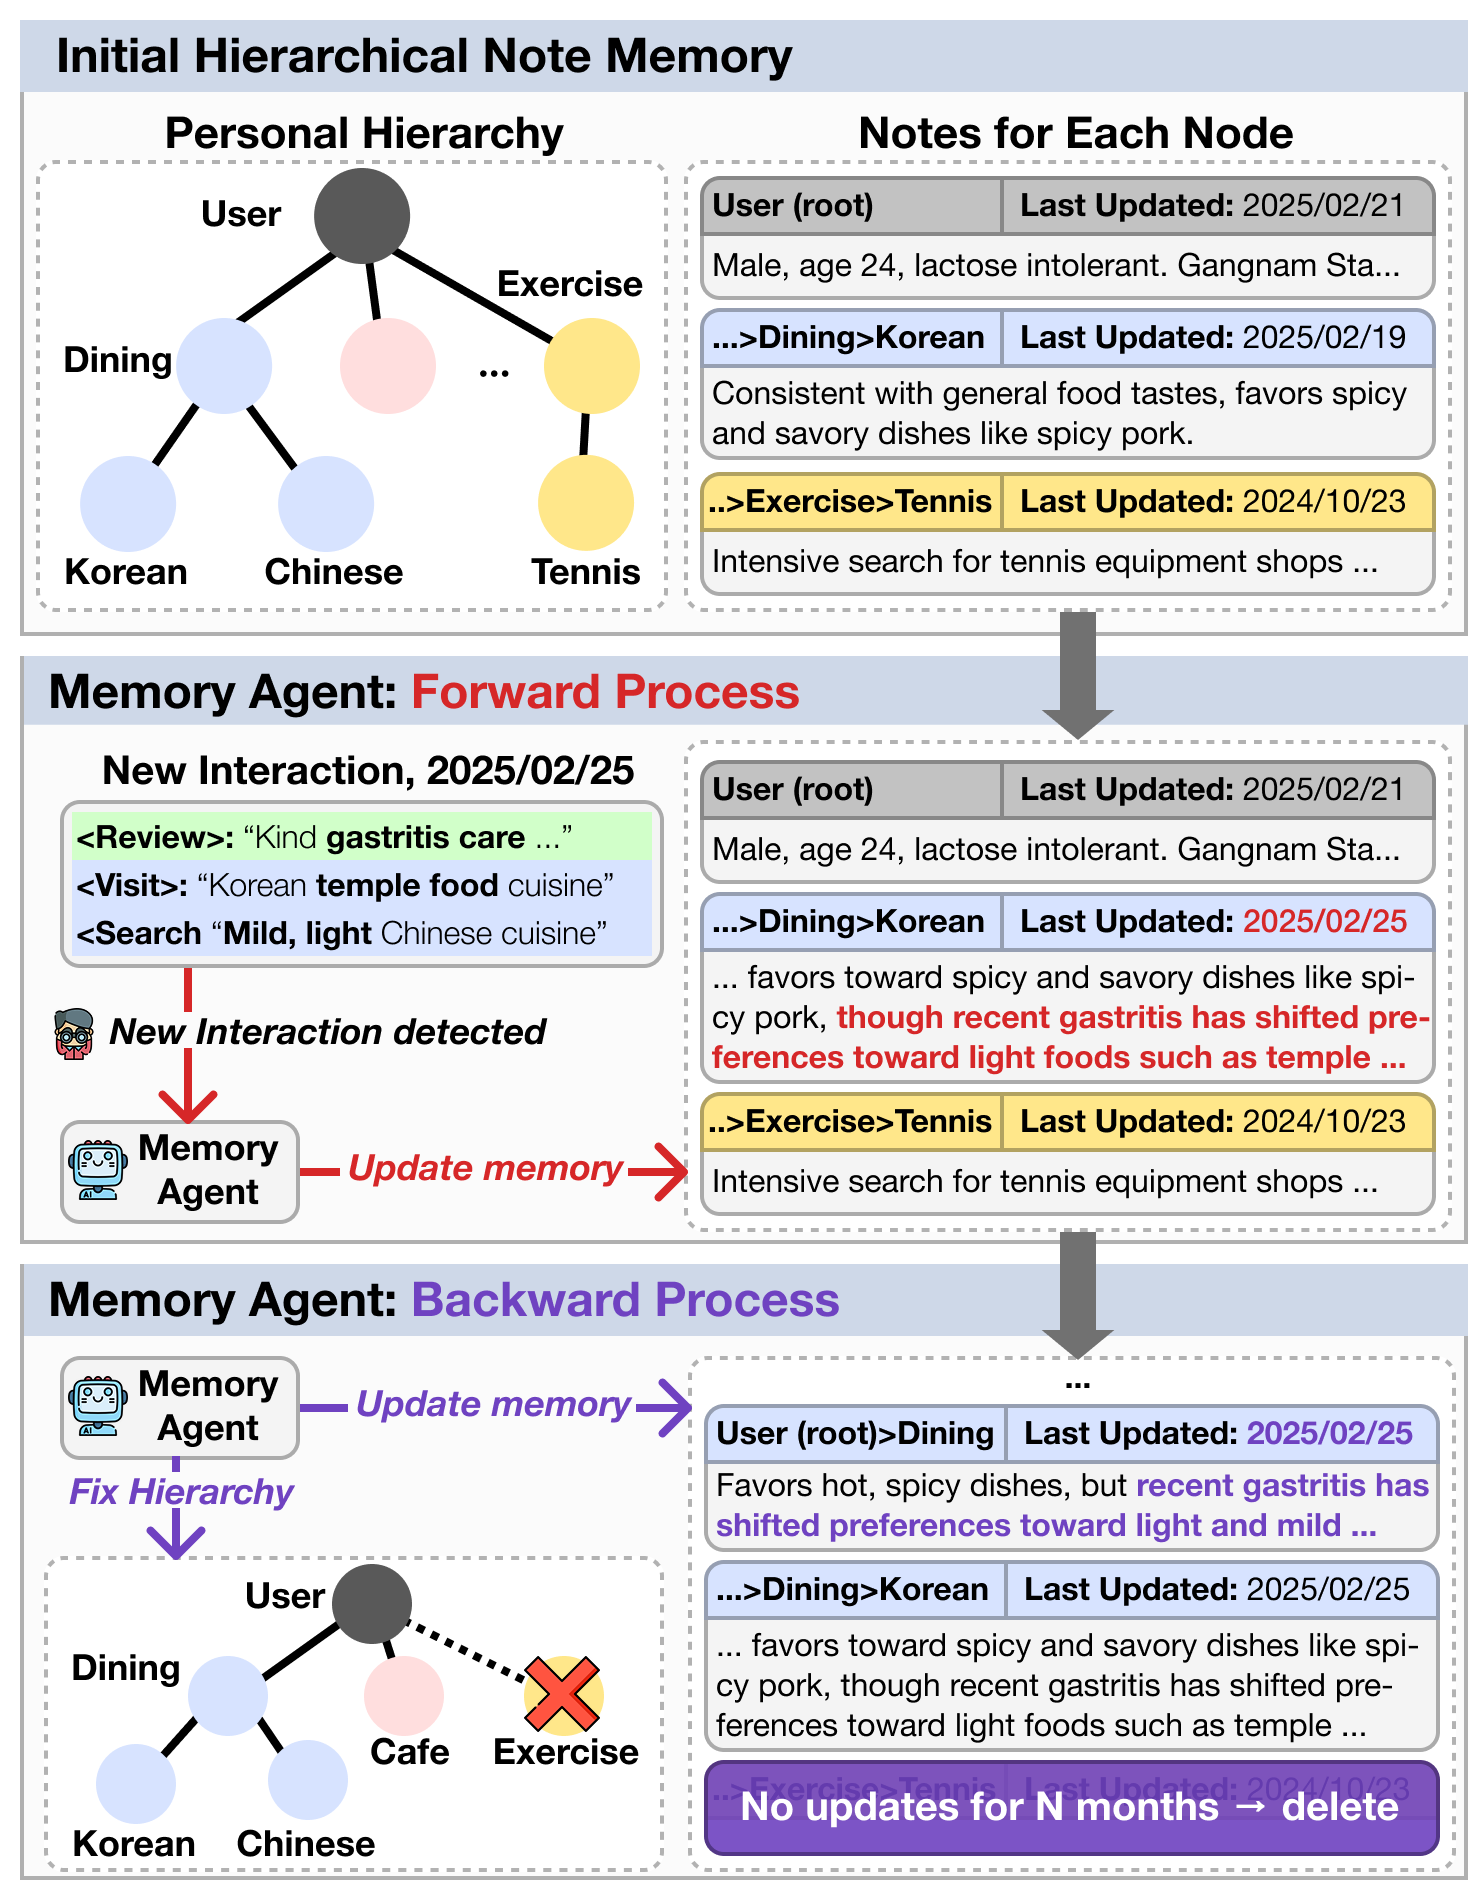
\includegraphics[width=\linewidth]{figures/method.png}
  \Description{Diagram of the Memory Agent operation in three stages: an initial per-node note tree anchored to a personal hierarchy, a forward update where a new interaction selectively modifies only the affected Korean-cuisine note, and a backward consolidation step where a shared trait is elevated from child to parent with concrete subcategory words preserved at the child while stale leaves are pruned.}
  \caption{Memory Agent operation. \textit{Initial}: per-node notes anchored to a personal hierarchy (the root demographic note shown here has since been removed). \textit{Forward}: a new interaction selectively updates only the affected note (Korean). \textit{Backward}: a shared trait is elevated from child to parent while concrete subcategory words stay at the child, and stale leaves are pruned. This is the \emph{intended} backward behaviour; Section~\ref{sec:loss} measures how often the deployed system achieves it.}
  \label{fig:workflow}
\end{figure}


Each node in the hierarchy is associated with a \textit{Note}, a structured record holding the accumulated preference knowledge for that category:

\begin{itemize}
    \item \textbf{path}: the full hierarchical path (e.g., ``User $>$ Dining $>$ Korean Food''),
    \item \textbf{summary}: a natural-language paragraph summarizing the user's preferences and behavioral patterns for this category, integrating both explicit and implicit signals (e.g., for the Korean Food node: ``favors spicy and savory dishes such as spicy pork,'' inferred from repeated visits and supportive review excerpts),
    \item \textbf{keywords}: BM25-oriented keyword tags for retrieval,
    \item \textbf{updated\_count}: the number of times the note content has been substantively modified,
    \item \textbf{recently\_updated}: the date of the most recent content update (e.g., the Korean Food note advances from 2025/02/19 to 2025/02/25 after new activity arrives, while the Tennis note, last updated on 2024/10/23, remains unchanged).
\end{itemize}

A sixth field, \textbf{user\_info}, held demographic and factual attributes at the root (e.g., ``24-year-old male, lactose intolerant, frequently active near Gangnam Station''). Root-exclusivity was requested in the routing prompt but, like depth, was never enforced in code. The field was removed from the API response, then from the pipeline, then from the stored data during the period covered by this paper; Section~\ref{sec:governance} gives the reason. The snapshots our measurements run on predate the removal, and \(6.5\%\) of their notes carry a non-empty value.

All notes for a user are stored atomically in a single Parquet file, enabling efficient bulk I/O. Tree structure metadata (parent--child relationships, node levels) is kept in a separate hierarchy file, so the Memory Agent can load, modify, and persist the entire memory state in one read-modify-write cycle per operation.

\section{Stale leaf pruning}
\label{app:pruning}

A leaf node \(n\) is pruned when it satisfies both conditions simultaneously:
\begin{equation}
\label{eq:pruning}
    \mathrm{updates}(n) \leq \tau_u \quad \text{and} \quad \mathrm{age}(n) > \tau_d,
\end{equation}
where \(\mathrm{updates}(n)\) is the cumulative update count (the schema field \texttt{updated\_count}), \(\mathrm{age}(n)\) is days since its last update, \(\tau_u\) is the minimum update threshold (default 2), and \(\tau_d\) the staleness threshold in days (default 120). Nodes are processed in decreasing depth order, so pruning a leaf may expose its parent as a new leaf, which is then evaluated in the same pass. The mechanism keeps one-off exploratory behaviour from accumulating while retaining nodes reinforced by repeated interaction.

\section{Held-out MCQ construction}
\label{app:mcq}

The target is each user's first qualified review in 2026-07-16..08-20, strictly after the 2026-07-15 snapshot the memory was built from. Distractors are three same-category POIs matched on review count (\(999/1000\) within \(\pm 20\%\)), excluding anything the user has touched, with sensitive categories dropped to match deployed routing.

Target availability, not tree eligibility, is the binding constraint: review availability retains only \(44.8\%\) of the partition against tree eligibility's \(99.2\%\). We therefore filter on the target first and balance strata within what survives, and require one review in the window rather than our earlier rule's five, which would have retained \(1.5\%\) of this cohort. The distractors are matched on category and review count but not on distance from the user, which Section~\ref{sec:delivery} treats as a measured confound rather than a controlled one.

\section{Signal extraction detail}
\label{app:extraction}

User preferences for places appear through two different channels: explicit signals written by the user, and implicit signals inferred from behavior. We extract a structured preference profile from each channel separately, then merge them in the hierarchical memory. Separating the two channels suits the POI domain, where implicit behavioral signals are abundant but ambiguous and explicit ones are sparse but precise. A third demographic axis is introduced later, during forward aggregation (Section~\ref{sec:forward}), with root-exclusive routing.

\paragraph{Explicit Signal Extraction.}
Explicit signals originate from user-authored content (primarily place reviews), where preferences are stated directly in natural language (e.g., ``I love spicy broth'' or ``the quiet atmosphere was perfect for working''). We process review histories with an LLM-based extraction pipeline that, for each user, produces a set of structured persona items. Each item consists of four fields: (a)~\textit{User\_Info}, a single atomic fact about the user's lifestyle or preference distilled from the review evidence; (b)~\textit{Rationale}, a chain-of-thought justification grounded in specific review dates, place names, and quoted expressions; (c)~\textit{User\_Vocabulary}, verbatim words and phrases from the user's original text to preserve linguistic identity; and (d)~\textit{Reference}, indices into the source review records.

To handle the wide variance in review volume across users, we employ two few-shot prompt strategies: a \textit{rich} variant with detailed examples for users who have written many reviews, and a \textit{sparse} variant with conservative, observation-oriented examples for users with limited review data. The sparse strategy deliberately avoids over-generalizing from insufficient evidence, instead emphasizing factual descriptions of observed behavior.

\paragraph{Implicit Signal Extraction.}
Implicit signals are derived from non-verbal behavioral traces: search queries, POI clicks, dwell patterns, and place saves. Unlike reviews, these actions do not directly articulate preferences, but consistent patterns across many interactions can reveal latent interests~\cite{proex}. We construct a profiling pipeline that transforms raw click logs into structured personas through the following steps:

\begin{enumerate}
    \item \textbf{Sessionization.} Consecutive interactions involving the same query or the same POI within a 60-minute window are grouped into micro-sessions. Each session records the query text, timestamps, day of week, clicked POI name and category, location, review popularity rank, and click count.

    \item \textbf{Demographic context attachment.} Available demographic attributes (age, gender, marital status, household composition, occupation, and children information) are prepended to the session log as structured metadata. These attributes were later routed exclusively to the root node's \texttt{user\_info} field during hierarchical path mapping (Section~\ref{sec:forward}), enforcing a clean separation between demographic facts and behavioral preferences.

    \item \textbf{LLM-based persona profiling.} The sessionized log is passed to an LLM with strict constraints: (a)~all persona claims must cite specific click evidence; (b)~hallucination of unobserved behaviors (e.g., inferring residence from visit locations) is prohibited; (c)~stereotypical reasoning based on demographics is forbidden; and (d)~the output must decompose preferences into predefined POI domains (dining, caf\'{e}s, travel, medical, beauty, shopping, etc.).
\end{enumerate}

The output is a domain-partitioned persona string, where each domain section describes the user's inferred preferences with concrete behavioral evidence. To capture temporal dynamics, we apply this extraction over sliding windows (e.g., 21-day periods) across the observation period and aggregate the per-window results into a unified implicit persona per user.


\section{Forward aggregation detail}
\label{app:forward}

When new interaction data arrives (either explicit persona extractions or implicit persona profiles), the Memory Agent executes a three-step forward pass to integrate the information into the existing memory. Each step is mediated by an LLM call; for a user with $N$ distinct target paths identified in Step~2, the total cost is
\begin{equation}
\#\mathrm{LLM\,calls}(u) \;=\; 2 + N(u),
\end{equation}
where the constant $2$ accounts for the single extraction call (Step~1) and the single path-mapping call (Step~2), and Step~3 contributes one call per target path.

\paragraph{Step~1: Preference Profile Extraction.}
The raw interaction text, combining both implicit behavioral profiles and explicit review extractions, is analyzed by an LLM to separate three categories of information:

\begin{itemize}
    \item \textbf{User information} ($\mathcal{U}$): objective, slowly-changing facts such as age, occupation, and primary activity region.
    \item \textbf{Explicit preferences} ($\mathcal{P}_e$): stated preferences where the user directly expresses likes, dislikes, or requirements in language (e.g., ``I prefer acidic coffee'' or ``I look for outlets at caf\'{e}s'').
    \item \textbf{Implicit preferences} ($\mathcal{P}_i$): latent preferences inferred from non-verbal behavioral patterns (e.g., ``tends toward isolated, productivity-oriented spaces'' derived from repeated clicks on quiet study caf\'{e}s).
\end{itemize}

This three-axis separation isolates demographic facts into a dedicated channel. The LLM is instructed to preserve concrete keywords from the source data rather than abstracting them (e.g., extracting specific dish names rather than ``diverse menu''), to merge semantically similar items into compact statements, and to strictly distinguish between exploratory actions (clicks, searches) and confirmed actions (visits, reservations) to avoid inflating behavioral claims.

\paragraph{Step~2: Hierarchical Path Mapping.}
Unlike learned taxonomy expansion such as TaxoExpan~\cite{taxoexpan}, our routing is performed in-context by an LLM that jointly considers base-taxonomy paths and any user-specific paths created in earlier sessions. The mapping enforces five principles: \textit{(i)~root exclusivity for demographics}---while the field existed, $\mathcal{U}$ items were mapped only to the root \texttt{user\_info} field, never as subcategory nodes; \textit{(ii)~context-aware routing}---``prefers quiet atmosphere'' goes to ``User $>$ Caf\'{e}'' if surrounding evidence is caf\'{e}-related, otherwise to the root; \textit{(iii)~semantic reuse}---existing paths are preferred when they subsume the new item (a ``latte'' preference maps to ``Coffee/Tea'' rather than a new ``Latte'' sibling); \textit{(iv)~hierarchical consistency}---new Level-3 nodes must match the abstraction level of their siblings (``Korean''/``Japanese'' under ``Dining'' yes; ``Naengmyeon'' no, it belongs under ``Korean''), and nodes at Level~4 or deeper are prohibited; \textit{(v)~aggregation}---items targeting the same path are grouped into one update call.

\paragraph{Step~3: Note Update.}
For each target path, an LLM acts as an \textit{editor} rather than appender~\cite{mem0}: it compares new data with existing content, resolves conflicts in favor of recency, removes outdated entries, and consolidates redundant statements. The root node managed demographics in its \texttt{user\_info} field (since removed; Section~\ref{sec:governance}); sub-nodes are restricted to category-specific preferences. Substantive changes increment \texttt{updated\_count} and refresh \texttt{recently\_updated}.

\section{Guard wording}
\label{app:guard}
The prompts are Korean; the rendering below is ours. The deployed guard is one instruction appended to the elevation prompt: proper nouns --- place names, store names, brands --- are kept verbatim at the child and never lifted to the parent. The wording derived from the measured loss profile (guard-v2) replaces it with:

\begin{quote}\small
\textbf{Preserve concrete nouns.} Never abstract or delete the following; leave them verbatim in the child note: (1) names of categories, business types and kinds of food (e.g., Korean, Chinese, Japanese, gukbap, fried chicken, jokbal, sushi, izakaya, bakery, caf\'{e}, grilled meat, raw fish); (2) place, store and brand names; (3) behavioural-evidence phrases (e.g., repeated clicks, repeated searches, sustained interest, saved POIs). Do not replace them with umbrella terms such as ``diverse food'' or ``dining preference''. State at the parent only the tendency the children share, and do not move a child's concrete nouns to the parent.
\end{quote}

%% ============================================================
%% REFERENCES
%% ============================================================
\bibliographystyle{ACM-Reference-Format}

\begingroup
\footnotesize
\begin{thebibliography}{99}
\setlength{\itemsep}{0pt}
\setlength{\parskip}{0pt}

\bibitem{maynez-faithfulness}
J.~Maynez, S.~Narayan, B.~Bohnet, and R.~McDonald.
\newblock On faithfulness and factuality in abstractive summarization.
\newblock In \textit{ACL}, 2020.

\bibitem{hallucination-survey}
L.~Huang, W.~Yu, W.~Ma, W.~Zhong, Z.~Feng, H.~Wang, Q.~Chen, W.~Peng, X.~Feng, B.~Qin, and T.~Liu.
\newblock A survey on hallucination in large language models: Principles, taxonomy, challenges, and open questions.
\newblock \textit{ACM Transactions on Information Systems}, 2025. arXiv:2311.05232.

\bibitem{llmlingua}
H.~Jiang, Q.~Wu, C.-Y.~Lin, Y.~Yang, and L.~Qiu.
\newblock {LLMLingua}: Compressing prompts for accelerated inference of large language models.
\newblock In \textit{EMNLP}, 2023. arXiv:2310.05736.

\bibitem{formatspread}
M.~Sclar, Y.~Choi, Y.~Tsvetkov, and A.~Suhr.
\newblock Quantifying language models' sensitivity to spurious features in prompt design, or: How {I} learned to start worrying about prompt formatting.
\newblock In \textit{ICLR}, 2024. arXiv:2310.11324.

\bibitem{multiprompt}
M.~Mizrahi, G.~Kaplan, D.~Malkin, R.~Dror, D.~Shahaf, and G.~Stanovsky.
\newblock State of what art? {A} call for multi-prompt {LLM} evaluation.
\newblock \textit{Transactions of the ACL}, 12, 2024.

\bibitem{memory-survey}
Z.~Zhang, X.~Bo, C.~Ma, R.~Li, X.~Chen, Q.~Dai, J.~Zhu, Z.~Dong, and J.-R.~Wen.
\newblock A survey on the memory mechanism of large language model based agents.
\newblock \textit{arXiv preprint arXiv:2404.13501}, 2024.

\bibitem{mtbench}
L.~Zheng, W.-L.~Chiang, Y.~Sheng, S.~Zhuang, Z.~Wu, Y.~Zhuang, Z.~Lin, Z.~Li, D.~Li, E.~P.~Xing, H.~Zhang, J.~E.~Gonzalez, and I.~Stoica.
\newblock Judging {LLM-as-a-Judge} with {MT-Bench} and {Chatbot Arena}.
\newblock In \textit{NeurIPS Datasets and Benchmarks Track}, 2023.

\bibitem{laaj-survey}
J.~Gu, X.~Jiang, Z.~Shi, H.~Tan, X.~Zhai, C.~Xu, W.~Li, Y.~Shen, S.~Ma, H.~Liu, S.~Wang, K.~Zhang, Y.~Wang, W.~Gao, L.~Ni, and J.~Guo.
\newblock A survey on {LLM-as-a-Judge}.
\newblock \textit{arXiv preprint arXiv:2411.15594}, 2025.

\bibitem{laaj-podcast}
F.~Fabbri, G.~Penha, E.~D'Amico, A.~Wang, M.~De~Nadai, J.~Doremus, P.~Gigioli, A.~Damianou, O.~St{\aa}l, and M.~Lalmas.
\newblock Evaluating podcast recommendations with profile-aware {LLM-as-a-Judge}.
\newblock In \textit{RecSys}, 2025. arXiv:2508.08777.

\bibitem{qwen3}
A.~Yang, A.~Yang, B.~Zhang, B.~Hui, B.~Zheng, B.~Yu, C.~Li, D.~Liu, F.~Huang, G.~Dong, et~al.
\newblock {Qwen3} technical report.
\newblock \textit{arXiv preprint arXiv:2505.09388}, 2025.

\bibitem{vllm}
W.~Kwon, Z.~Li, S.~Zhuang, Y.~Sheng, L.~Zheng, C.~H.~Yu, J.~E.~Gonzalez, H.~Zhang, and I.~Stoica.
\newblock Efficient memory management for large language model serving with {PagedAttention}.
\newblock In \textit{SOSP}, 2023.

\bibitem{personamem-v2}
B.~Jiang, Y.~Yuan, M.~Shen, Z.~Hao, Z.~Xu, Z.~Chen, Z.~Liu, A.~R.~Vijjini, J.~He, H.~Yu, R.~Poovendran, G.~Wornell, L.~Ungar, D.~Roth, S.~Chen, and C.~J.~Taylor.
\newblock {PersonaMem-v2}: Towards personalized intelligence via learning implicit user personas and agentic memory.
\newblock \textit{arXiv preprint arXiv:2512.06688}, 2025.

\bibitem{personamem}
B.~Jiang, Z.~Hao, Y.-M.~Cho, B.~Li, Y.~Yuan, S.~Chen, L.~Ungar, C.~J.~Taylor, and D.~Roth.
\newblock Know me, respond to me: Benchmarking {LLMs} for dynamic user profiling and personalized responses at scale.
\newblock In \textit{COLM}, 2025. arXiv:2504.14225.

\bibitem{mem0}
P.~Chhikara, D.~Khant, S.~Aryan, T.~Singh, and D.~Yadav.
\newblock Mem0: Building production-ready {AI} agents with scalable long-term memory.
\newblock \textit{arXiv preprint arXiv:2504.19413}, 2025.

\bibitem{amem}
W.~Xu, Z.~Liang, K.~Mei, H.~Gao, J.~Tan, and Y.~Zhang.
\newblock {A-MEM}: Agentic memory for {LLM} agents.
\newblock In \textit{NeurIPS}, 2025. arXiv:2502.12110.

\bibitem{emem}
S.~Zhou and J.~Han.
\newblock A simple yet strong baseline for long-term conversational memory of {LLM} agents.
\newblock \textit{arXiv preprint arXiv:2511.17208}, 2025.

\bibitem{memgpt}
C.~Packer, S.~Wooders, K.~Lin, V.~Fang, S.~G.~Patil, I.~Stoica, and J.~E.~Gonzalez.
\newblock MemGPT: Towards {LLMs} as operating systems.
\newblock \textit{arXiv preprint arXiv:2310.08560}, 2023.

\bibitem{beyond-context-window}
N.~Pollertlam and W.~Kornsuwannawit.
\newblock Beyond the context window: A cost-performance analysis of fact-based memory vs.\ long-context {LLMs} for persistent agents.
\newblock \textit{arXiv preprint arXiv:2603.04814}, 2026.

\bibitem{lost-in-the-middle}
N.~F.~Liu, K.~Lin, J.~Hewitt, A.~Paranjape, M.~Bevilacqua, F.~Petroni, and P.~Liang.
\newblock Lost in the middle: How language models use long contexts.
\newblock \textit{Transactions of the ACL}, 2024.

\bibitem{personahub}
T.~Ge, X.~Chan, X.~Wang, D.~Yu, H.~Mi, and D.~Yu.
\newblock Scaling synthetic data creation with 1,000,000,000 personas.
\newblock \textit{arXiv preprint arXiv:2406.20094}, 2024.

\bibitem{personagym}
V.~Samuel et~al.
\newblock PersonaGym: Evaluating persona agents and {LLMs}.
\newblock In \textit{Findings of EMNLP}, 2025. arXiv:2407.18416.

\bibitem{personabench}
J.~Tan, L.~Yang, Z.~Liu, Z.~Liu, R.~Murthy, T.~M.~Awalgaonkar, J.~Zhang, W.~Yao, M.~Zhu, S.~Kokane, S.~Savarese, H.~Wang, C.~Xiong, and S.~Heinecke.
\newblock PersonaBench: Evaluating {AI} models on understanding personal information through accessing (synthetic) private user data.
\newblock In \textit{Findings of ACL}, 2025. arXiv:2502.20616.

\bibitem{synthesizeme}
M.~J.~Ryan, O.~Shaikh, A.~Bhagirath, D.~Frees, W.~Held, and D.~Yang.
\newblock SynthesizeMe! Inducing persona-guided prompts for personalized reward models in {LLMs}.
\newblock In \textit{ACL}, 2025. arXiv:2506.05598.

\bibitem{proex}
Y.~Zhang, Y.~Zhang, Y.~Wang, T.~Chen, and H.~Yin.
\newblock ProEx: A unified framework leveraging large language model with profile extrapolation for recommendation.
\newblock In \textit{KDD}, 2026. arXiv:2512.00679.

\bibitem{zeropoirec}
S.~Feng, H.~Lyu, C.~Chen, and Y.-S.~Ong.
\newblock Where to move next: Zero-shot generalization of {LLMs} for next {POI} recommendation.
\newblock \textit{arXiv preprint arXiv:2404.01855}, 2024.

\bibitem{persona-db}
C.~Sun, K.~Yang, R.~G.~Reddy, Y.~R.~Fung, H.~P.~Chan, K.~Small, C.~Zhai, and H.~Ji.
\newblock Persona-DB: Efficient large language model personalization for response prediction with collaborative data refinement.
\newblock \textit{arXiv preprint arXiv:2402.11060}, 2024.

\bibitem{rmm}
Z.~Tan, J.~Yan, I.-H.~Hsu, R.~Han, Z.~Wang, L.~T.~Le, Y.~Song, Y.~Chen, H.~Palangi, G.~Lee, A.~Iyer, T.~Chen, H.~Liu, C.-Y.~Lee, and T.~Pfister.
\newblock In prospect and retrospect: Reflective memory management for long-term personalized dialogue agents.
\newblock In \textit{ACL}, 2025. arXiv:2503.08026.

\bibitem{personax}
Y.~Shi, W.~Xu, Z.~Zhang, X.~Zi, Q.~Wu, and M.~Xu.
\newblock PersonaX: A recommendation agent oriented user modeling framework for long behavior sequence.
\newblock In \textit{Findings of ACL}, 2025. arXiv:2503.02398.

\bibitem{dpr}
V.~Karpukhin et~al.
\newblock Dense passage retrieval for open-domain question answering.
\newblock In \textit{Proceedings of EMNLP}, 2020.

\bibitem{contriever}
G.~Izacard et~al.
\newblock Unsupervised dense information retrieval with contrastive learning.
\newblock \textit{TMLR}, 2022.

\bibitem{mdl}
P.~Gr{\"u}nwald.
\newblock \textit{The Minimum Description Length Principle}.
\newblock MIT Press, 2007.

\bibitem{react}
S.~Yao, J.~Zhao, D.~Yu, N.~Du, I.~Shafran, K.~Narasimhan, and Y.~Cao.
\newblock {ReAct}: Synergizing reasoning and acting in language models.
\newblock In \textit{ICLR}, 2023.

\bibitem{reflexion}
N.~Shinn, F.~Cassano, E.~Berman, A.~Gopinath, K.~Narasimhan, and S.~Yao.
\newblock Reflexion: Language agents with verbal reinforcement learning.
\newblock In \textit{NeurIPS}, 2023.

\bibitem{generative-agents}
J.~S.~Park, J.~C.~O'Brien, C.~J.~Cai, M.~R.~Morris, P.~Liang, and M.~S.~Bernstein.
\newblock Generative agents: Interactive simulacra of human behavior.
\newblock In \textit{UIST}, 2023.

\bibitem{rag}
P.~Lewis, E.~Perez, A.~Piktus, F.~Petroni, V.~Karpukhin, N.~Goyal, H.~K{\"u}ttler, M.~Lewis, W.-t.~Yih, T.~Rockt{\"a}schel, S.~Riedel, and D.~Kiela.
\newblock Retrieval-augmented generation for knowledge-intensive {NLP} tasks.
\newblock In \textit{NeurIPS}, 2020.

\bibitem{self-rag}
A.~Asai, Z.~Wu, Y.~Wang, A.~Sil, and H.~Hajishirzi.
\newblock {Self-RAG}: Learning to retrieve, generate, and critique through self-reflection.
\newblock In \textit{ICLR}, 2024.

\bibitem{sasrec}
W.-C.~Kang and J.~McAuley.
\newblock Self-attentive sequential recommendation.
\newblock In \textit{ICDM}, 2018.

\bibitem{bert4rec}
F.~Sun, J.~Liu, J.~Wu, C.~Pei, X.~Lin, W.~Ou, and P.~Jiang.
\newblock {BERT4Rec}: Sequential recommendation with bidirectional encoder representations from {Transformer}.
\newblock In \textit{CIKM}, 2019.

\bibitem{deepmove}
J.~Feng, Y.~Li, C.~Zhang, F.~Sun, F.~Meng, A.~Guo, and D.~Jin.
\newblock {DeepMove}: Predicting human mobility with attentional recurrent networks.
\newblock In \textit{WWW}, 2018.

\bibitem{p5}
S.~Geng, S.~Liu, Z.~Fu, Y.~Ge, and Y.~Zhang.
\newblock Recommendation as language processing ({RLP}): A unified pretrain, personalized prompt \& predict paradigm ({P5}).
\newblock In \textit{RecSys}, 2022.

\bibitem{tallrec}
K.~Bao, J.~Zhang, Y.~Zhang, W.~Wang, F.~Feng, and X.~He.
\newblock {TALLRec}: An effective and efficient tuning framework to align large language model with recommendation.
\newblock In \textit{RecSys}, 2023.

\bibitem{mmlu}
D.~Hendrycks, C.~Burns, S.~Basart, A.~Zou, M.~Mazeika, D.~Song, and J.~Steinhardt.
\newblock Measuring massive multitask language understanding.
\newblock In \textit{ICLR}, 2021.

\bibitem{memorybank}
W.~Zhong, L.~Guo, Q.~Gao, H.~Ye, and Y.~Wang.
\newblock {MemoryBank}: Enhancing large language models with long-term memory.
\newblock In \textit{Proceedings of AAAI}, 2024.

\bibitem{hipporag}
B.~J.~Guti\'errez, Y.~Shu, Y.~Gu, M.~Yasunaga, and Y.~Su.
\newblock {HippoRAG}: Neurobiologically inspired long-term memory for large language models.
\newblock In \textit{NeurIPS}, 2024.

\bibitem{lamp}
A.~Salemi, S.~Mysore, M.~Bendersky, and H.~Zamani.
\newblock {LaMP}: When large language models meet personalization.
\newblock In \textit{ACL}, 2024.

\bibitem{oppu}
Z.~Tan, Q.~Zeng, Y.~Tian, Z.~Liu, B.~Yin, and M.~Jiang.
\newblock Democratizing large language models via personalized parameter-efficient fine-tuning ({OPPU}).
\newblock In \textit{EMNLP}, 2024.

\bibitem{getnext}
S.~Yang, J.~Liu, and K.~Zhao.
\newblock {GETNext}: Trajectory flow map enhanced transformer for next {POI} recommendation.
\newblock In \textit{SIGIR}, 2022.

\bibitem{stan}
Y.~Luo, Q.~Liu, and Z.~Liu.
\newblock {STAN}: Spatio-temporal attention network for next location recommendation.
\newblock In \textit{WWW}, 2021.

\bibitem{llara}
J.~Liao, S.~Li, Z.~Yang, J.~Wu, Y.~Yuan, X.~Wang, and X.~He.
\newblock {LLaRA}: Large language-recommendation assistant.
\newblock In \textit{SIGIR}, 2024.

\bibitem{rankgpt}
W.~Sun, L.~Yan, X.~Ma, S.~Wang, P.~Ren, Z.~Chen, D.~Yin, and Z.~Ren.
\newblock Is {ChatGPT} good at search? {Investigating} large language models as re-ranking agents.
\newblock In \textit{EMNLP}, 2023.

\bibitem{ruler}
C.-P.~Hsieh, S.~Sun, S.~Kriman, S.~Acharya, D.~Rekesh, F.~Jia, Y.~Zhang, and B.~Ginsburg.
\newblock {RULER}: What's the real context size of your long-context language models?
\newblock \textit{arXiv preprint arXiv:2404.06654}, 2024.

\bibitem{llm4rec-survey}
L.~Wu, Z.~Zheng, Z.~Qiu, H.~Wang, H.~Gu, T.~Shen, C.~Qin, C.~Zhu, H.~Zhu, Q.~Liu, H.~Xiong, and E.~Chen.
\newblock A survey on large language models for recommendation.
\newblock \textit{World Wide Web}, 27, Article~60, 2024.

\bibitem{hydra}
Y.~Zhuang, H.~Sun, Y.~Yu, R.~Qiang, Q.~Wang, C.~Zhang, and B.~Dai.
\newblock {HYDRA}: Model factorization framework for black-box {LLM} personalization.
\newblock In \textit{NeurIPS}, 2024.

\bibitem{recmind}
Y.~Wang, Z.~Jiang, Z.~Chen, F.~Yang, Y.~Zhou, E.~Cho, X.~Fan, Y.~Lu, X.~Huang, and Y.~Yang.
\newblock {RecMind}: Large language model powered agent for recommendation.
\newblock In \textit{NAACL Findings}, 2024.

\bibitem{needle-haystack}
G.~Kamradt.
\newblock Needle in a haystack---pressure testing {LLM}s.
\newblock GitHub repository, \texttt{gkamradt/LLMTest\_NeedleInAHaystack}, 2023.

\bibitem{taxoexpan}
J.~Shen, Z.~Shen, C.~Xiong, C.~Wang, K.~Wang, and J.~Han.
\newblock {TaxoExpan}: Self-supervised taxonomy expansion with position-enhanced graph neural network.
\newblock In \textit{WWW}, 2020.

\end{thebibliography}
\endgroup

\end{document}
